\documentclass{article}
\usepackage{graphicx}
\graphicspath{{images/}}
\usepackage{layout}
\usepackage[a4paper, total={6in, 9in}]{geometry}
\usepackage[colorlinks = true,
            linkcolor = blue,
            urlcolor  = blue,
            citecolor = blue,
            anchorcolor = blue]{hyperref}%hiperenllaços
\usepackage[catalan]{babel}
\usepackage{minted} %Para el entorno de código
\usepackage[table,xcdraw]{xcolor}  %Para el color del entorno del código
\usepackage{enumitem}
\usepackage[T1]{fontenc}
\usepackage{setspace}
\usepackage{amsmath}
\usepackage{lipsum}
\usepackage{subfig}
\usepackage{hyperref}

\newcommand\myfontsize{\fontsize{13pt}{16pt}\selectfont}
\usemintedstyle{monokai}
\definecolor{mybgcolor}{RGB}{0,0,0} % Define el color de fondo deseado



\begin{document}

%TITOL
\begin{titlepage}
    \centering
    
\includegraphics[width=0.75\textwidth]{images/uib.png}\par\vspace{1cm}
    {\scshape\LARGE Grado de Ingeniería Informática \par}
    \vspace{1cm}
%Clasificación de la práctica
    {\Large Tecnologías Multimedia \par}
    \vspace{1.5cm}
%Titulo de la practica
    {\huge\bfseries Documentación Puertos Mallorca\par}
    \vspace{2cm}
%Autores / autor.
    {\large
    Jaume Adrover Fernández \\
    jaume.adrover3@estudiant.uib.cat \\
    \vspace{0.5cm}
    Marc Cañellas Gomez \\
    marc.canellas@estudiant.uib.cat \\
    \vspace{0.5cm}
    Diego Bermejo Cabañas \\
    diego.bermejo@estudiant.uib.cat \\
    \vspace{0.5cm}
    Joan Balaguer Llagostera \\
    joan.balaguer2@estudiant.uib.cat \\
    \textit{}\\
    \texttt{}
    \par}
    \vfill

% Bottom of the page
    {\large \texttt{} \\\today\par}
\end{titlepage}

\newpage
\hypersetup{linkcolor=black}
\tableofcontents
\newpage

\section{Introducción}
En este documento se explicará el contenido de la web-app que hemos desarrollado de forma que se pueda entender como se ha desarrollado. Además, se mostrarán todas sus funcionalidades para que el usuario tenga en cuenta todo lo que puede hacer con la web-app. Por otro lado, se explicarán que herramientas se han usado para el desarrollo de esta, además de las librerías, APIs y extras utilizados para la composición gráfica de la página.

\section{URL}
Primero de todo se mostrará como se puede acceder a la web-app desarrollada. En nuestro caso, hemos comprado un servicio de hosting en la página \href{https://www.dondominio.com/es/}{dondominio.com} gracias a los códigos proporcionados por nuestro profesor de la asignatura. En nuestro caso, hemos elegido como nombre de la URL para acceder a nuestra web-app \href{http://www.puertosmallorca.com/}{puertosmallorca.com}. Hemos elegido este nombre, ya que lo encontramos relativamente corto, conciso y muestra muy claramente lo que podrás encontrar en nuestra web-app. principalmente, lo hemos elegido siguiendo las recomendaciones que se nos especificaban en la página de contratación del hosting.

\section{Funcionalidades de la Web-App}
Una vez explicado como hemos contratado el servicio de hosting y podemos acceder a la web-app, mediante el link proporcionado en la sección anterior, pasaremos a explicar todas las funcionalidades que el usuario puede realizar con ella.

\subsection{Home Page}
Nada más entrar al link proporcionado, encontraremos una barra de navegación que se mantiene fija en la parte superior de la página. En la parte de la izquierda de esta, encontramos el logo y el nombre de la web-app y tanto el logo como el nombre, servirán para que el usuario pueda volver a la \textit{homepage} des cualquier desde de la web-app con tan solo clicar encima de una de ellas. En la parte de la derecha de la barra de navegación, encontramos 3 botones para acceder a las diferentes funcionalidades que ofrece la página:
\begin{itemize}
    \item \textbf{Ver Puertos}: este nos llevará más abajo de la \textit{homepage}, donde podremos obtener información sobre los puertos de Mallorca registrados en la página.
    \item \textbf{Contacto}: nos llevará a una página donde el usuario podrá contactar con nosotros en caso de tener cualquier problema.
\end{itemize}
\begin{figure}[ht]
    \centering
    
\includegraphics[width=0.95\textwidth]{images/nvbar.png}
    \caption{Barra de navegación de la web-app}
\end{figure}
Un poco más abajo de la barra de navegación, encontramos un carrusel de 3 fotos con textos encima de estas. En la primera de ellas se da la bienvenida al usuario, en la segunda, se muestra que puedes encontrar información sobre los puertos de mallorca y en la tercera que puedes crear tu plan de navegación. Con esto, damos a conocer de manera simple y concisa lo que el usuario puede hacer con nuestra web-app. El usuario se puede desplazar de forma manual por las fotos del carrusel, y también existe una flecha que apunta hacia abajo que nos llevará a la siguiente sección de la \textit{homepage}.
\newpage
\begin{figure}[ht]
    \centering
    \includegraphics[width=0.3\textwidth]{images/carousel1.png}
    \includegraphics[width=0.3\textwidth]{images/carousel2.png}
    \includegraphics[width=0.3\textwidth]{images/carousel3.png}
    \caption{Las 3 fotos del carrusel con sus respectivos textos}
\end{figure}

\noindent Una vez pasamos el carrusel de fotos, llegamos a la parte introductoria de la página, donde hay una pequeña descripción en forma de texto muy conocido sobre lo que se puede hacer en la página.
\begin{figure}[ht]
    \centering
    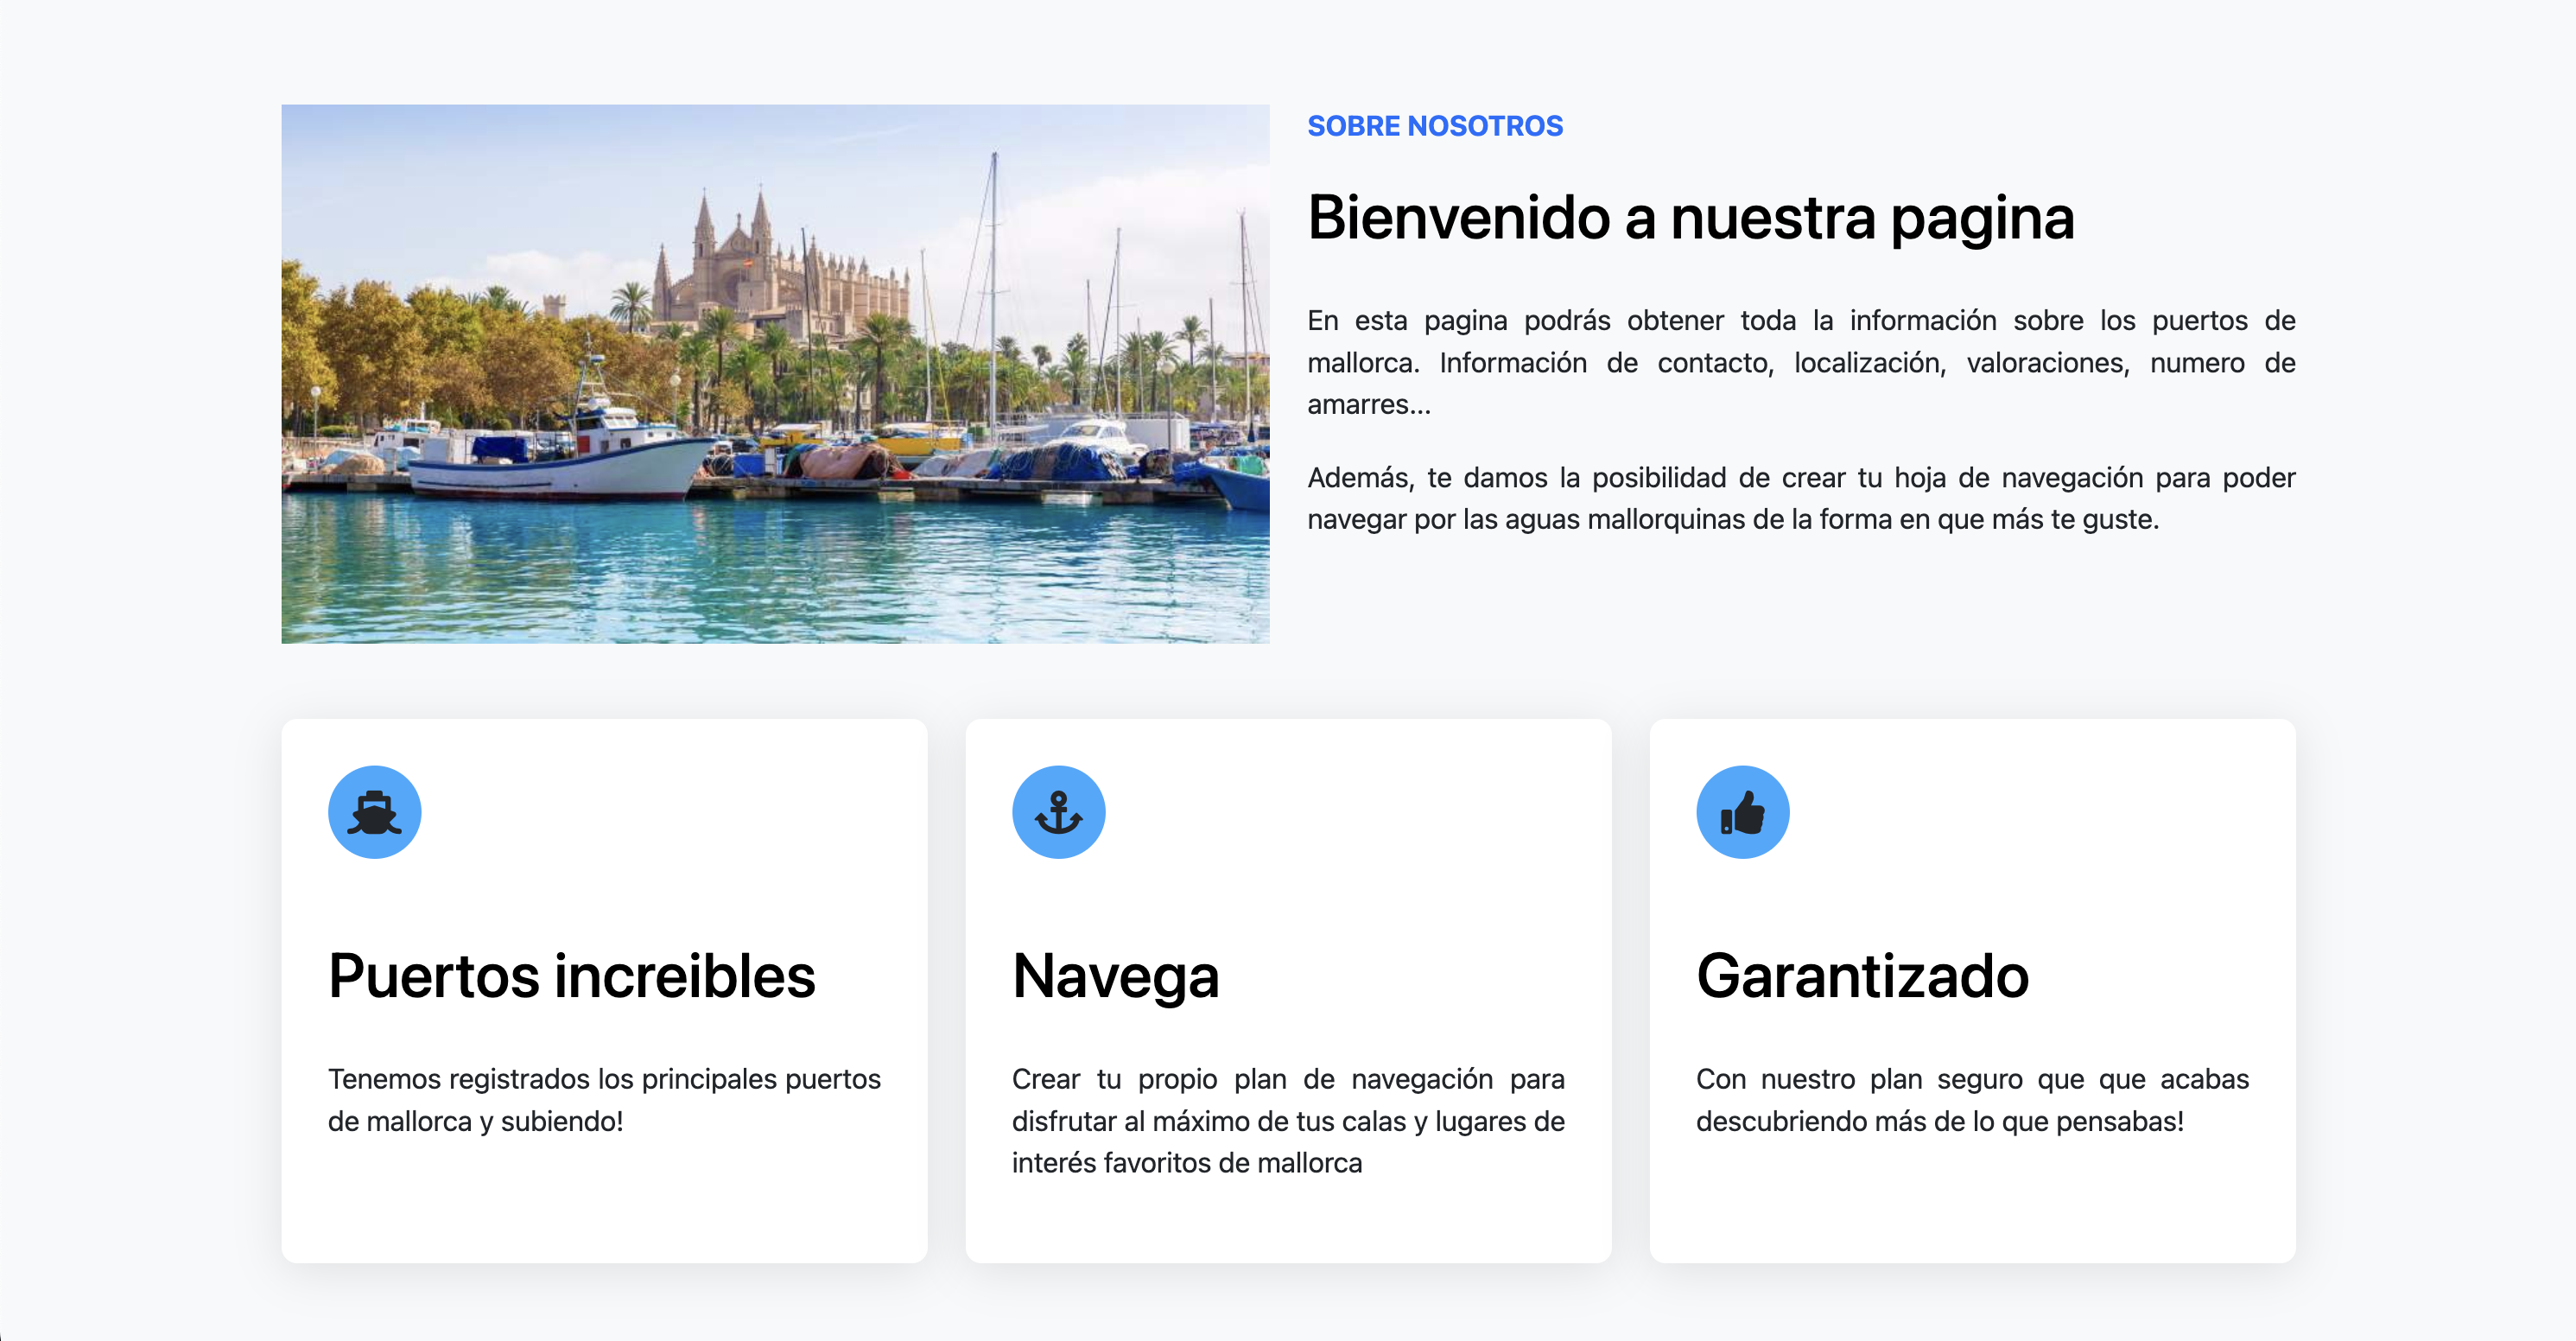
\includegraphics[width=0.7\textwidth]{images/introduccion.png}
    \caption{Sección introductoria de la web-app}
\end{figure}
\\Más abajo, encontramos la primera funcionalidad de nuestra web-app. Se muestra un mapa con marcadores rojos encima de los puertos registrados en la página. El mapa es interactivo, ya que se ha realizado mediante la API de Google Maps (la especificación técnica se explica más adelante en la documentación). Permite al usuario clicar encima de uno de los marcadores y así poder ver el nombre de este y, en caso de que el usuario quiera, tendrá un link que lo redirigirá a la página con la información del puerto seleccionado.
\begin{figure}[ht]
    \centering
    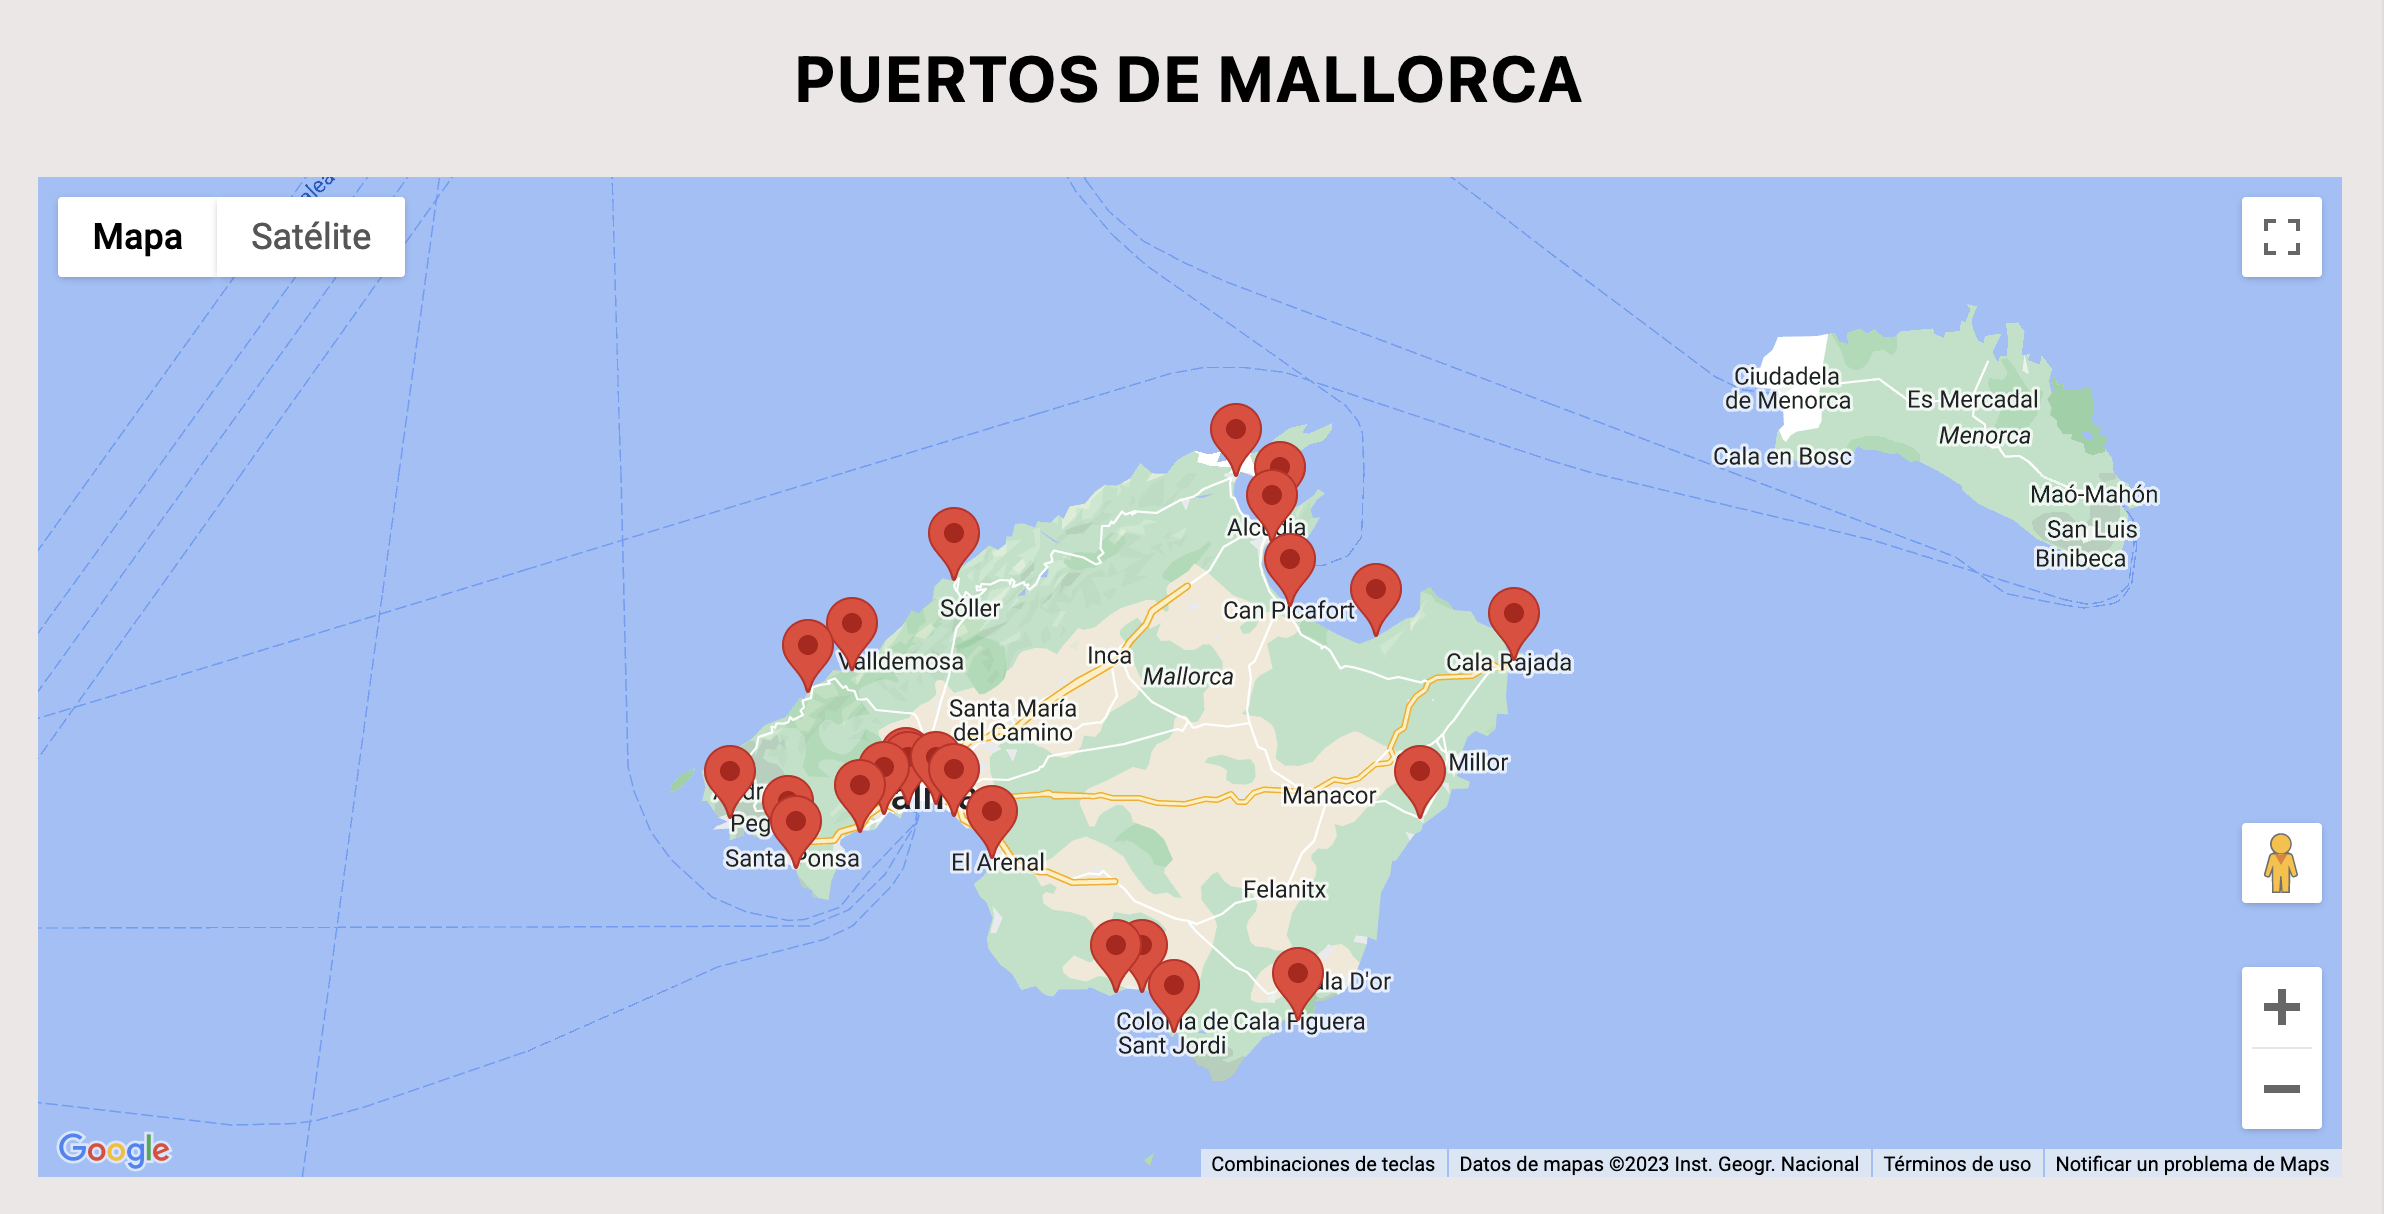
\includegraphics[width=0.75\textwidth]{images/mapa.png}
    \caption{Mapa interactivo de la web-app con todos los puertos disponibles en esta}
\end{figure}
\\Debajo del mapa, encontramos otra funcionalidad de la web-app. Mediante la barra de filtros, podemos tanto filtrar los puertos por sus características como ordenar los puertos buscados por una de sus características. De esta forma, el usuario podrá buscar los puertos con mayor capacidad, los de mayor valoración o incluso saber los puertos con capacidad mínima de 300 barcos.\\
\begin{figure}[ht]
    \centering
    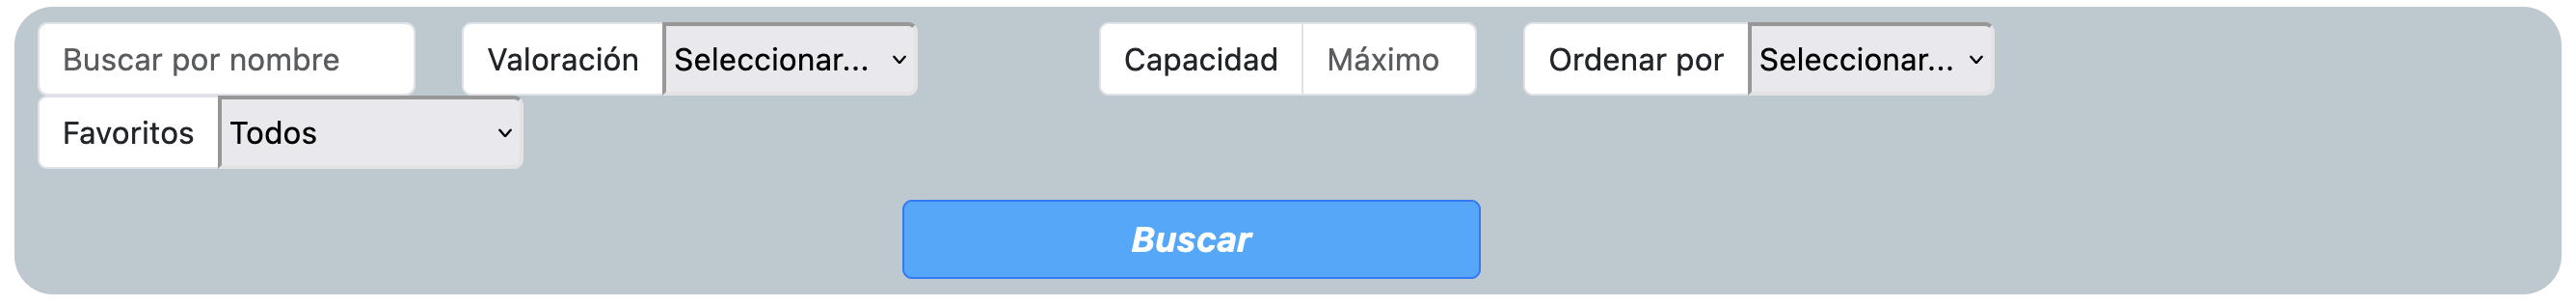
\includegraphics[width=1.0\textwidth]{images/filtros.png}
    \caption{Barra de filtros}
\end{figure}
\\Obviamente, la barra de filtros se aplica a las \texttt{cards} de los puertos que se muestran más abajo. En estas, se muestra su capacidad y su valoración en estrellas. También, si clicamos encima de la foto de uno de los puertos, nos redirigirá a la página del puerto en concreto.
\begin{figure}[ht]
    \centering
    \includegraphics[width=0.9\textwidth]{images/puertos.png}
    \caption{Ejemplos de \texttt{cards} donde se muestra una previsualización de los puertos}
\end{figure}
\\Para finalizar con la \textit{homepage}, encontramos el footer que encontramos en todas las sub páginas de nuestra web-app. En este, se muestran los nombres de los creadores de la página con sus respectivos links a sus páginas de GitHub, LinkedIn e Instagram.
\begin{figure}[ht]
    \centering
    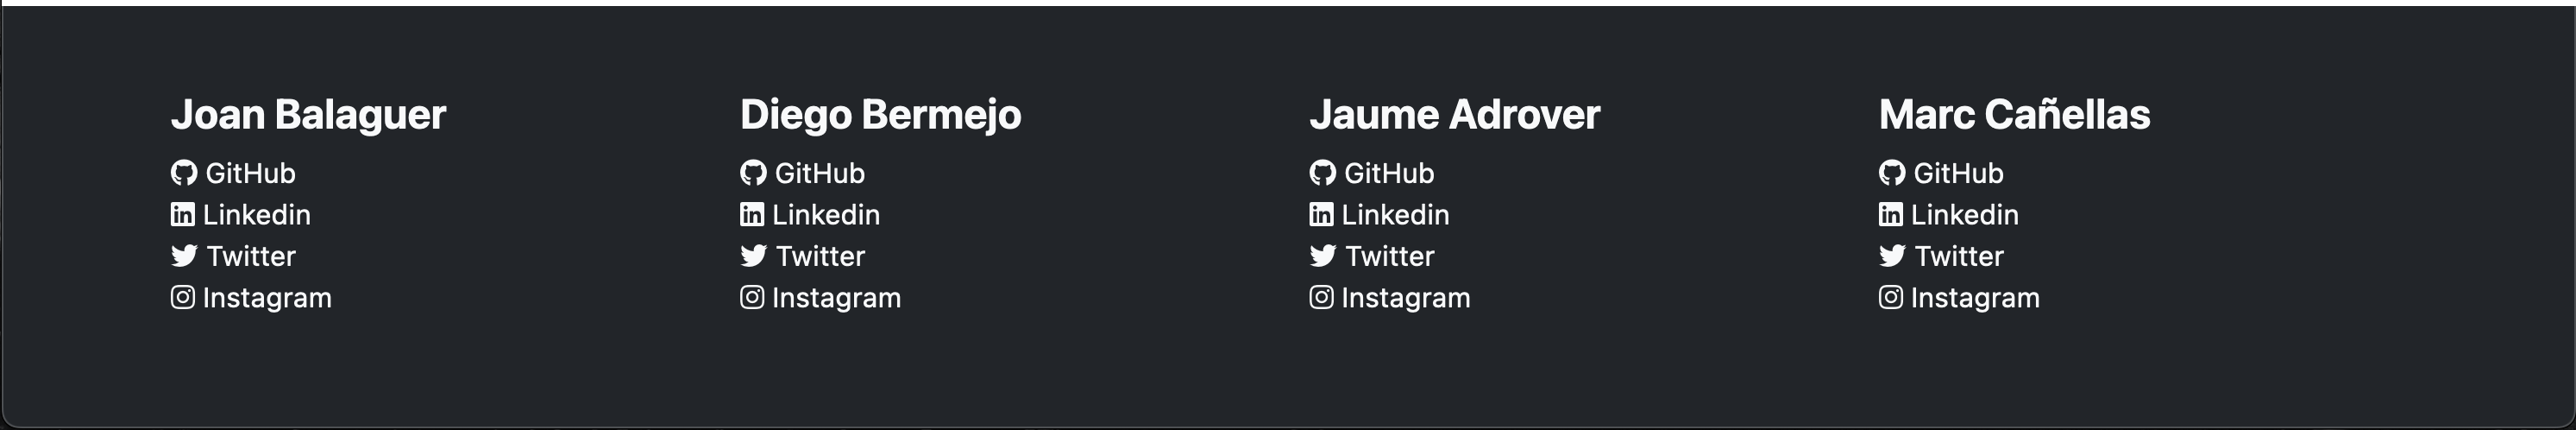
\includegraphics[width=0.9\textwidth]{images/footer.png}
    \caption{Footer de la web-app}
\end{figure}
\newpage
\subsection{Página de un Puerto}
Cuando seleccionamos uno de los puertos, la web-app nos redirige a la página con información del puerto. Esta tiene diversas partes:
\begin{itemize}
    \item \textbf{Título}: simplemente muestra el nombre del puerto seleccionado en grande en la parte superior de la página.
    \begin{figure}[ht]
        \centering
        
\includegraphics[width=0.7\textwidth]{images/tituloPuerto.png}
        \caption{Seccion donde se muestra el titulo del puerto (en este caso el de pollença)}
    \end{figure}
    \item \textbf{Descripción y video}: muestra el atributo de la descripción del puerto, además del video que tiene también como atributo.
    \begin{figure}[ht]
        \centering
        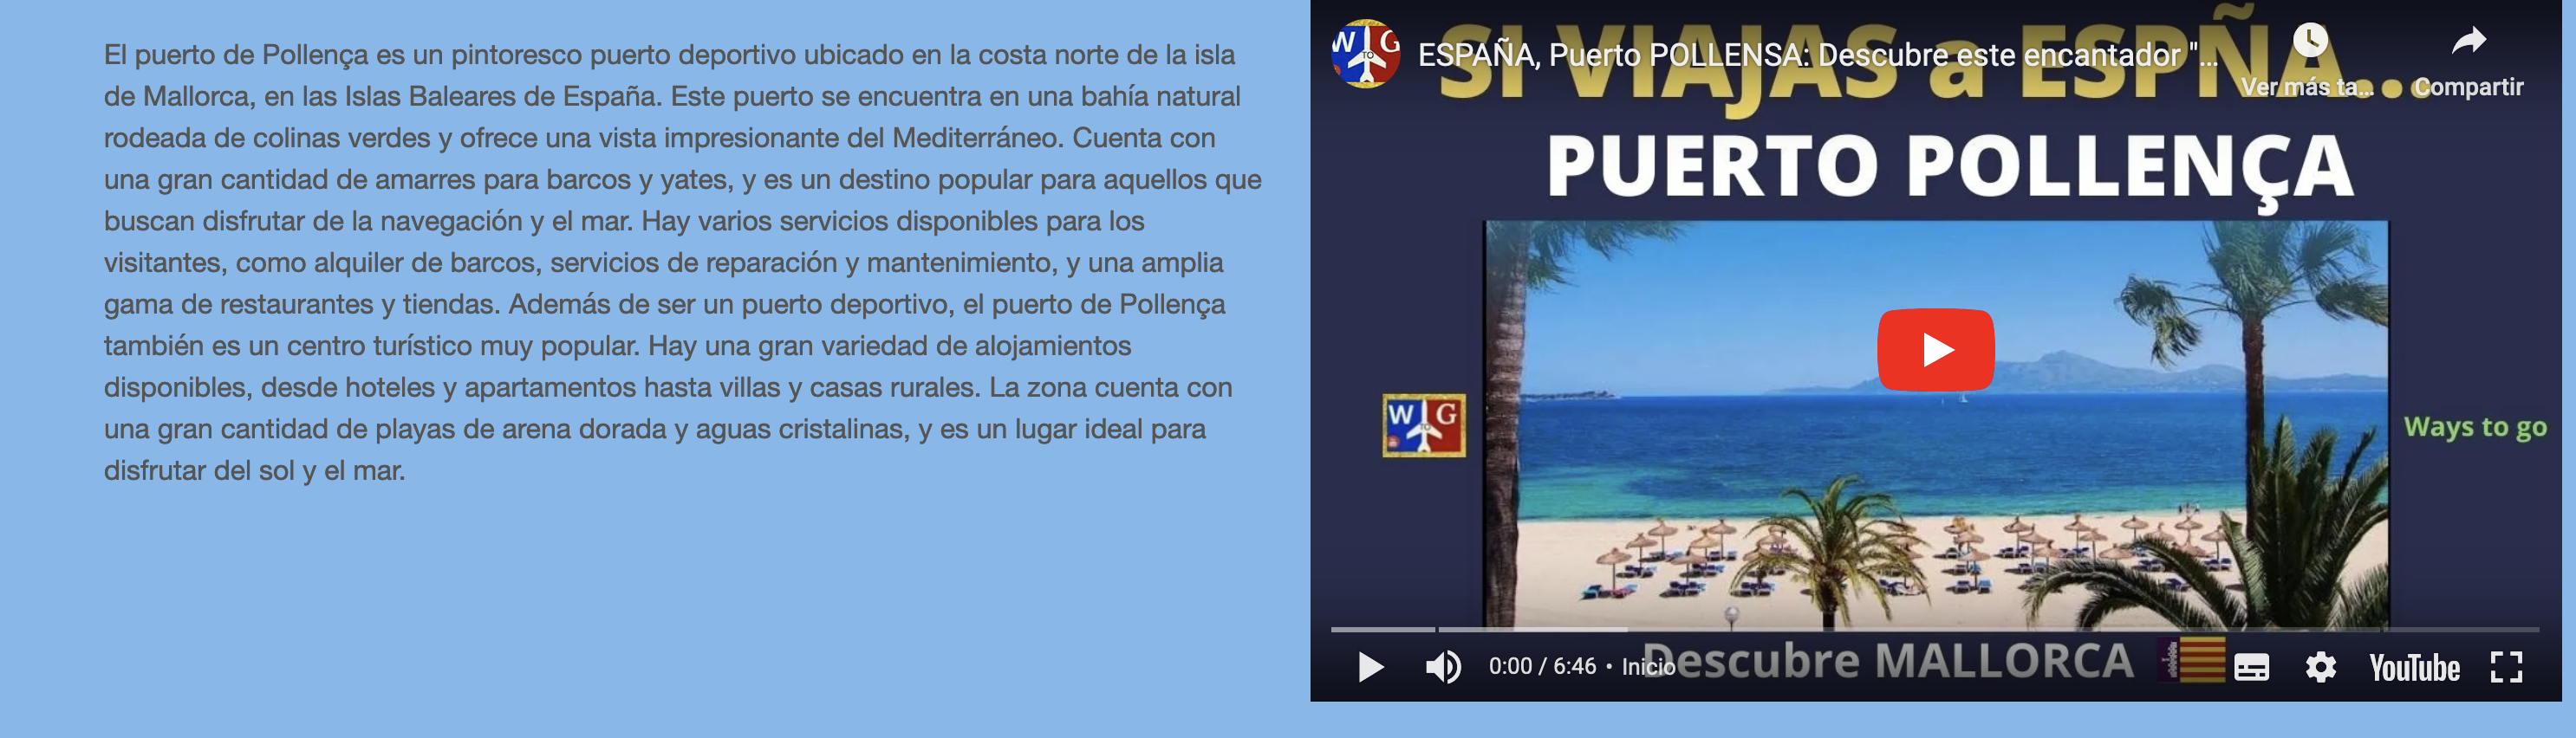
\includegraphics[width=0.7\textwidth]{images/descVid.png}
        \caption{Seccion donde se muestra la descripción del puerto junto al viodeo de youtube del puerto}
    \end{figure}
    \item \textbf{Características}: Muestra de forma concisa las características del puerto seleccionado. Se muestra su capacidad, su horario de apertura, si se permite fumar o no, la dirección, el correo electrónico, el teléfono y la valoración del puerto.
    \begin{figure}[ht]
        \centering
        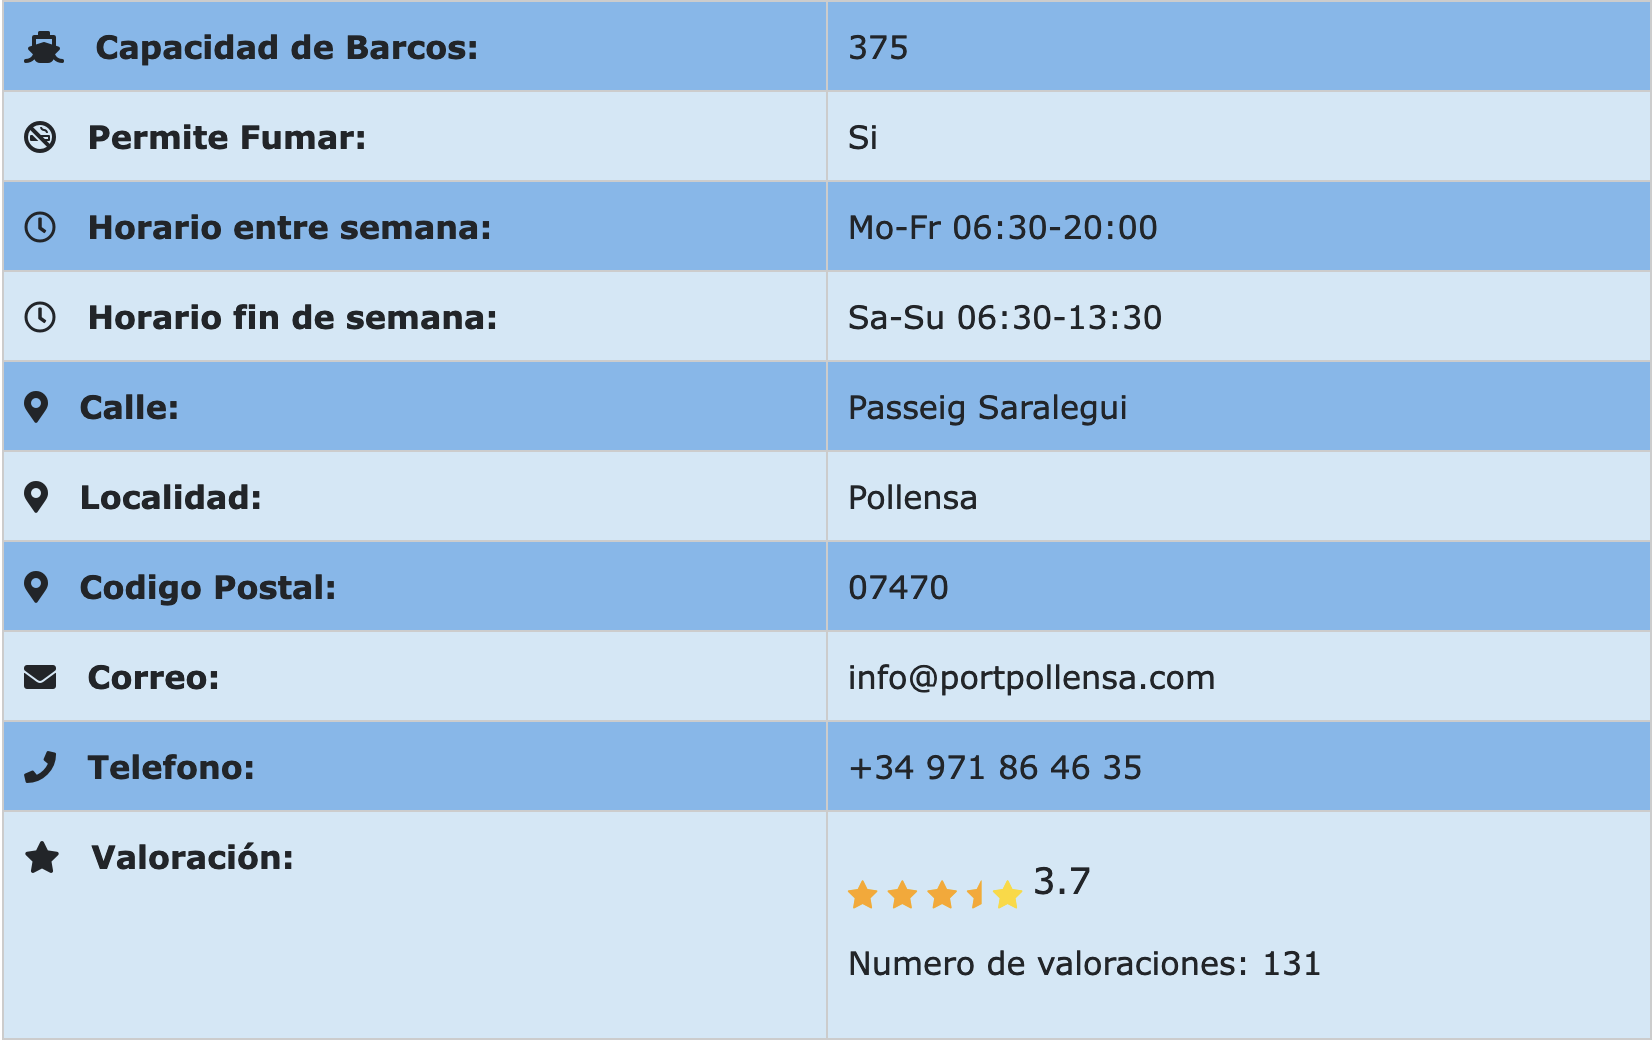
\includegraphics[width=0.7\textwidth]{images/caracteristicas.png}
        \caption{Sección donde se muestran los atributos propios de ese puerto en concreto}
    \end{figure}
    \newpage
    \item \textbf{Tiempo}: en este apartado se muestra el tiempo que hace en ese puerto en concreto.
    \begin{figure}[ht]
        \centering
        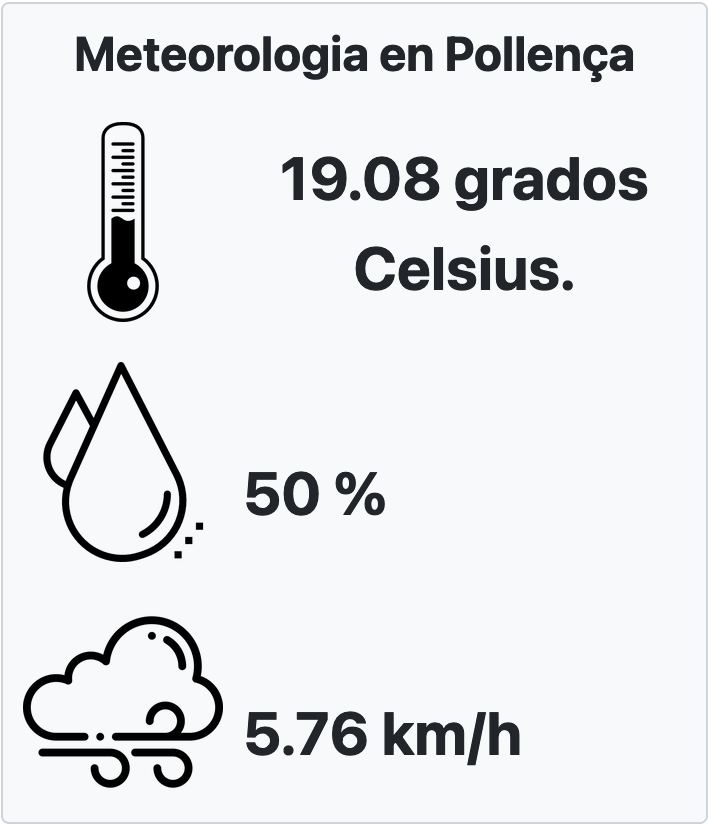
\includegraphics[width=0.3\textwidth]{images/tiempo.png}
        \caption{Sección donde se muestran el tiempo en el puerto}
    \end{figure}
    \item \textbf{Galería de Imágenes}: se muestran las imágenes que tenga como atributo el puerto seleccionado en el fichero json.
    \begin{figure}[ht]
        \centering
        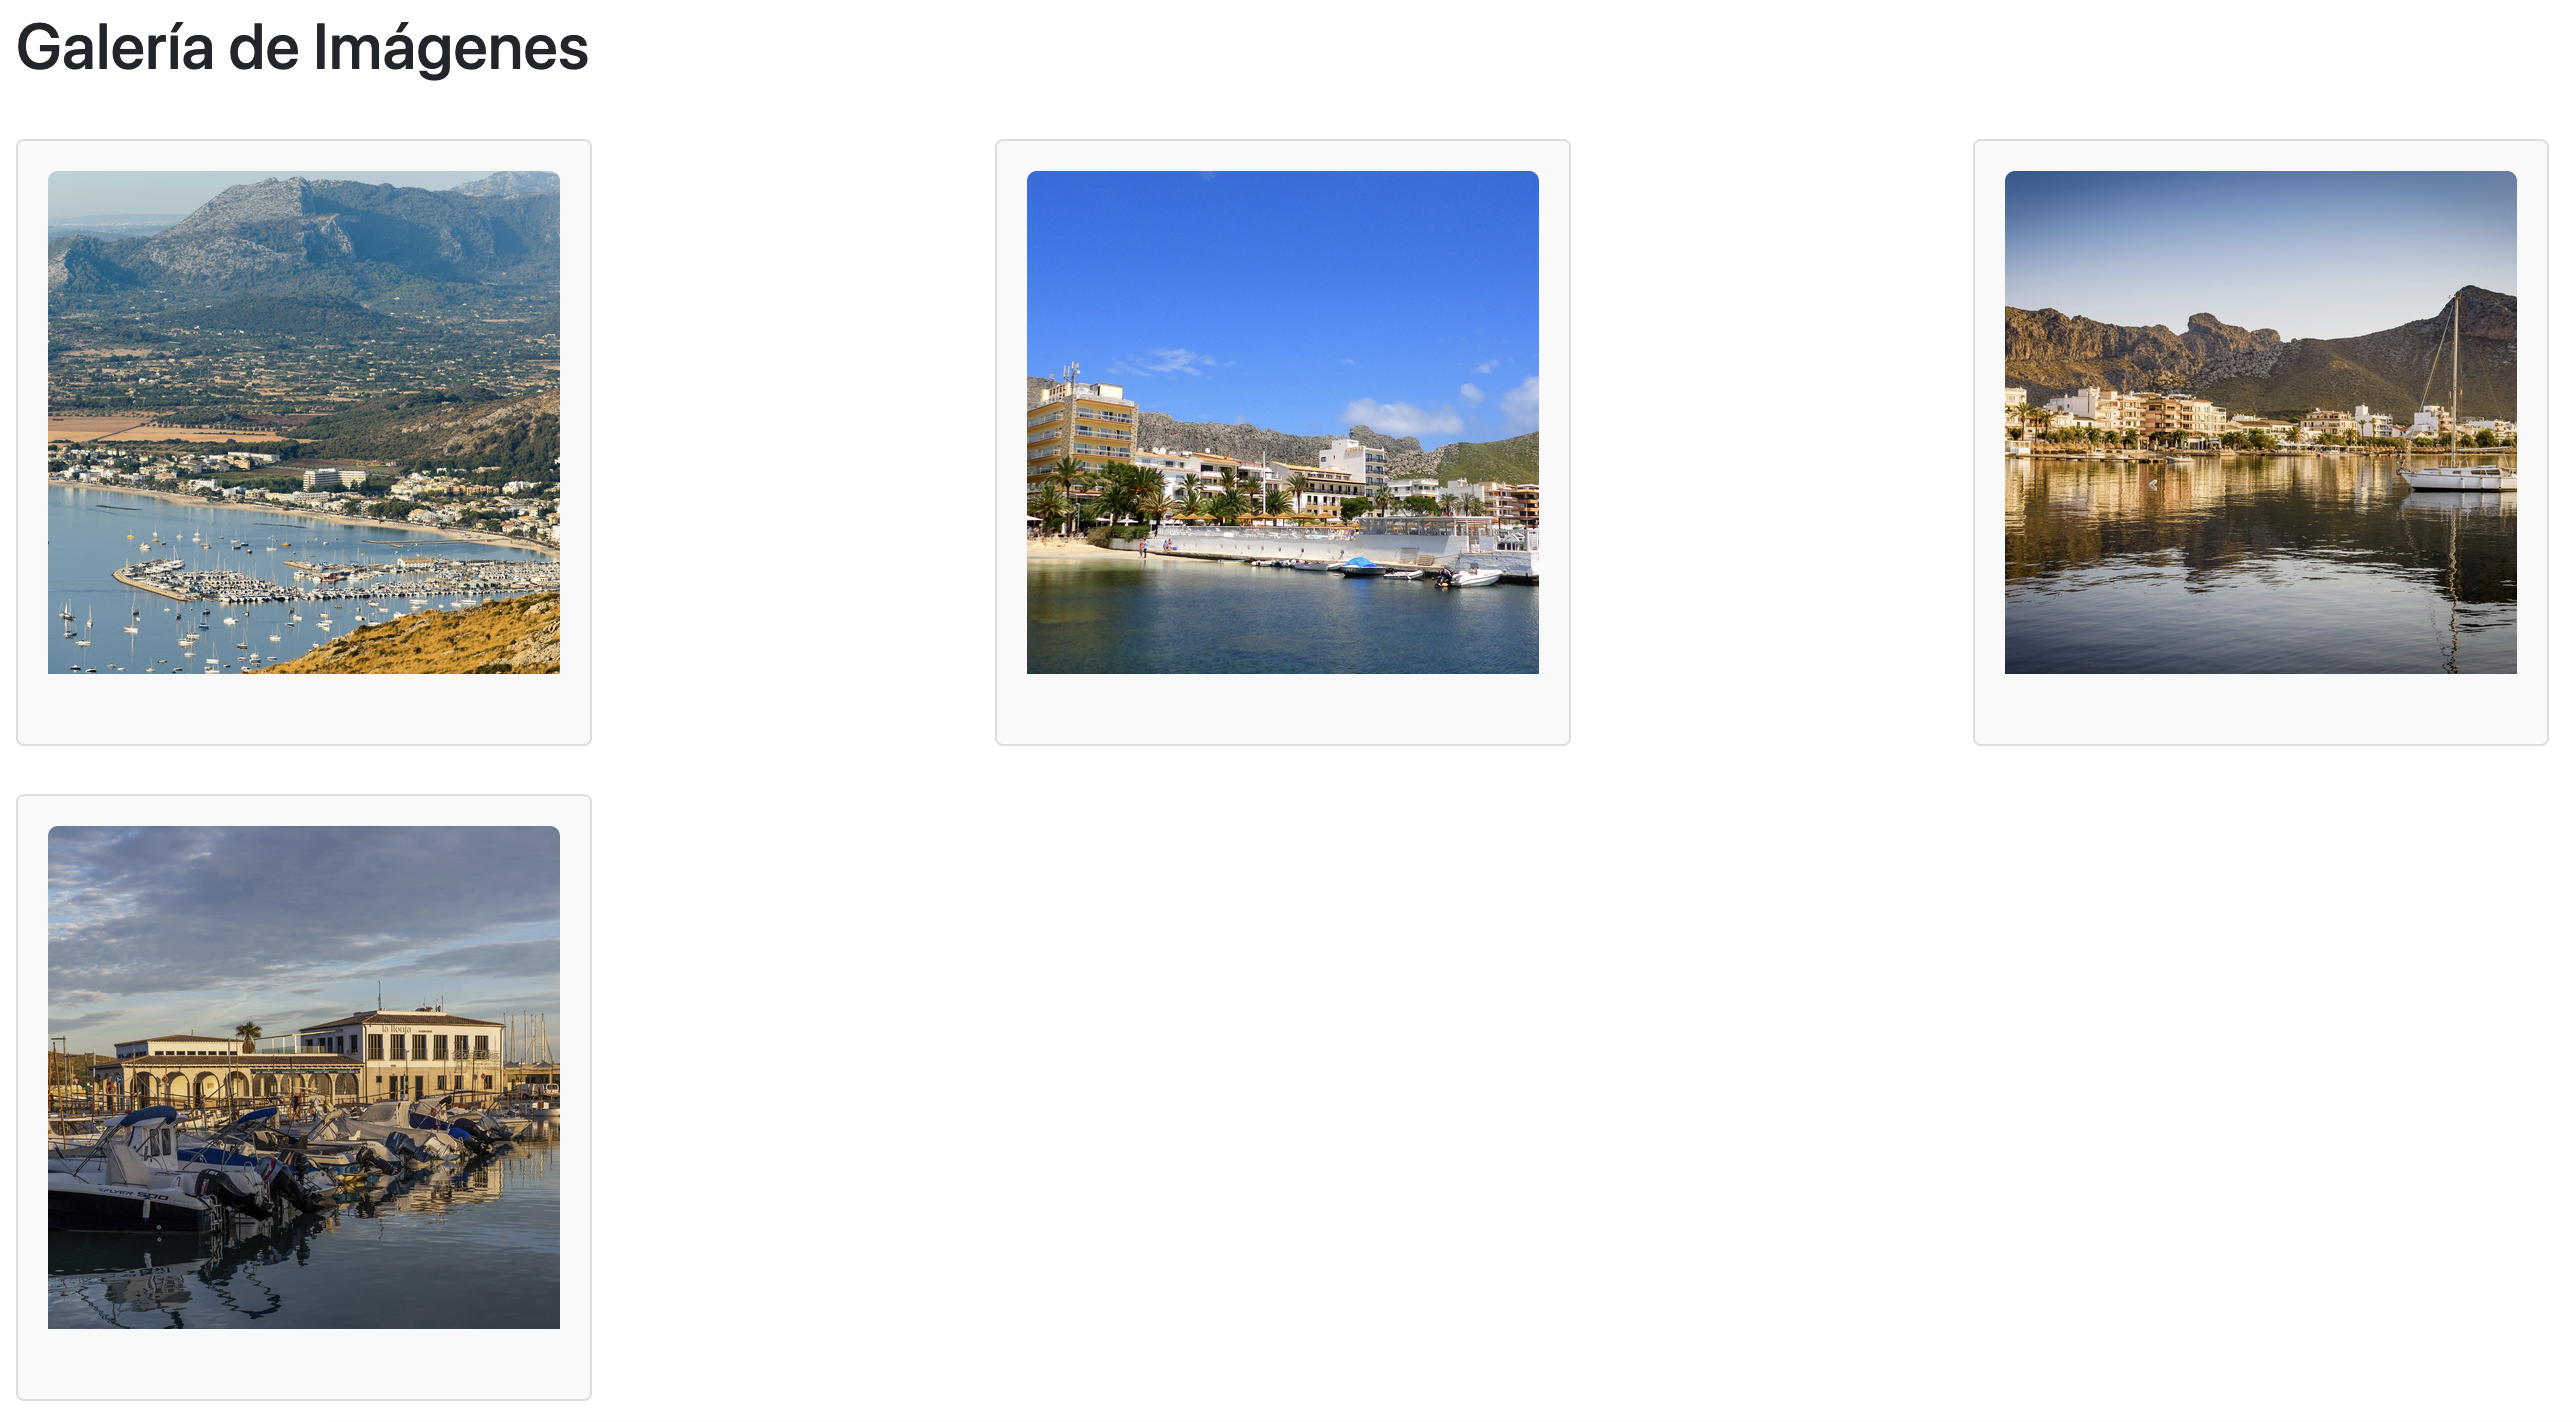
\includegraphics[width=0.5\textwidth]{images/galeriaImg.png}
        \caption{Footer de la web-app}
    \end{figure}
    \item \textbf{Lugares de interés cercanos}: sección en la cual se mostraran las playas, restaurantes y otros puertos cercanos. Contendrá dos partes principales. Por un lado, un mapa en el cual se mostraran en este los restaurantes i playas mas proximos al puerto y una segunda sección donde se mostraran unas \texttt{cards} con los puertos más cercanos.
    \begin{figure}[ht]
        \centering
        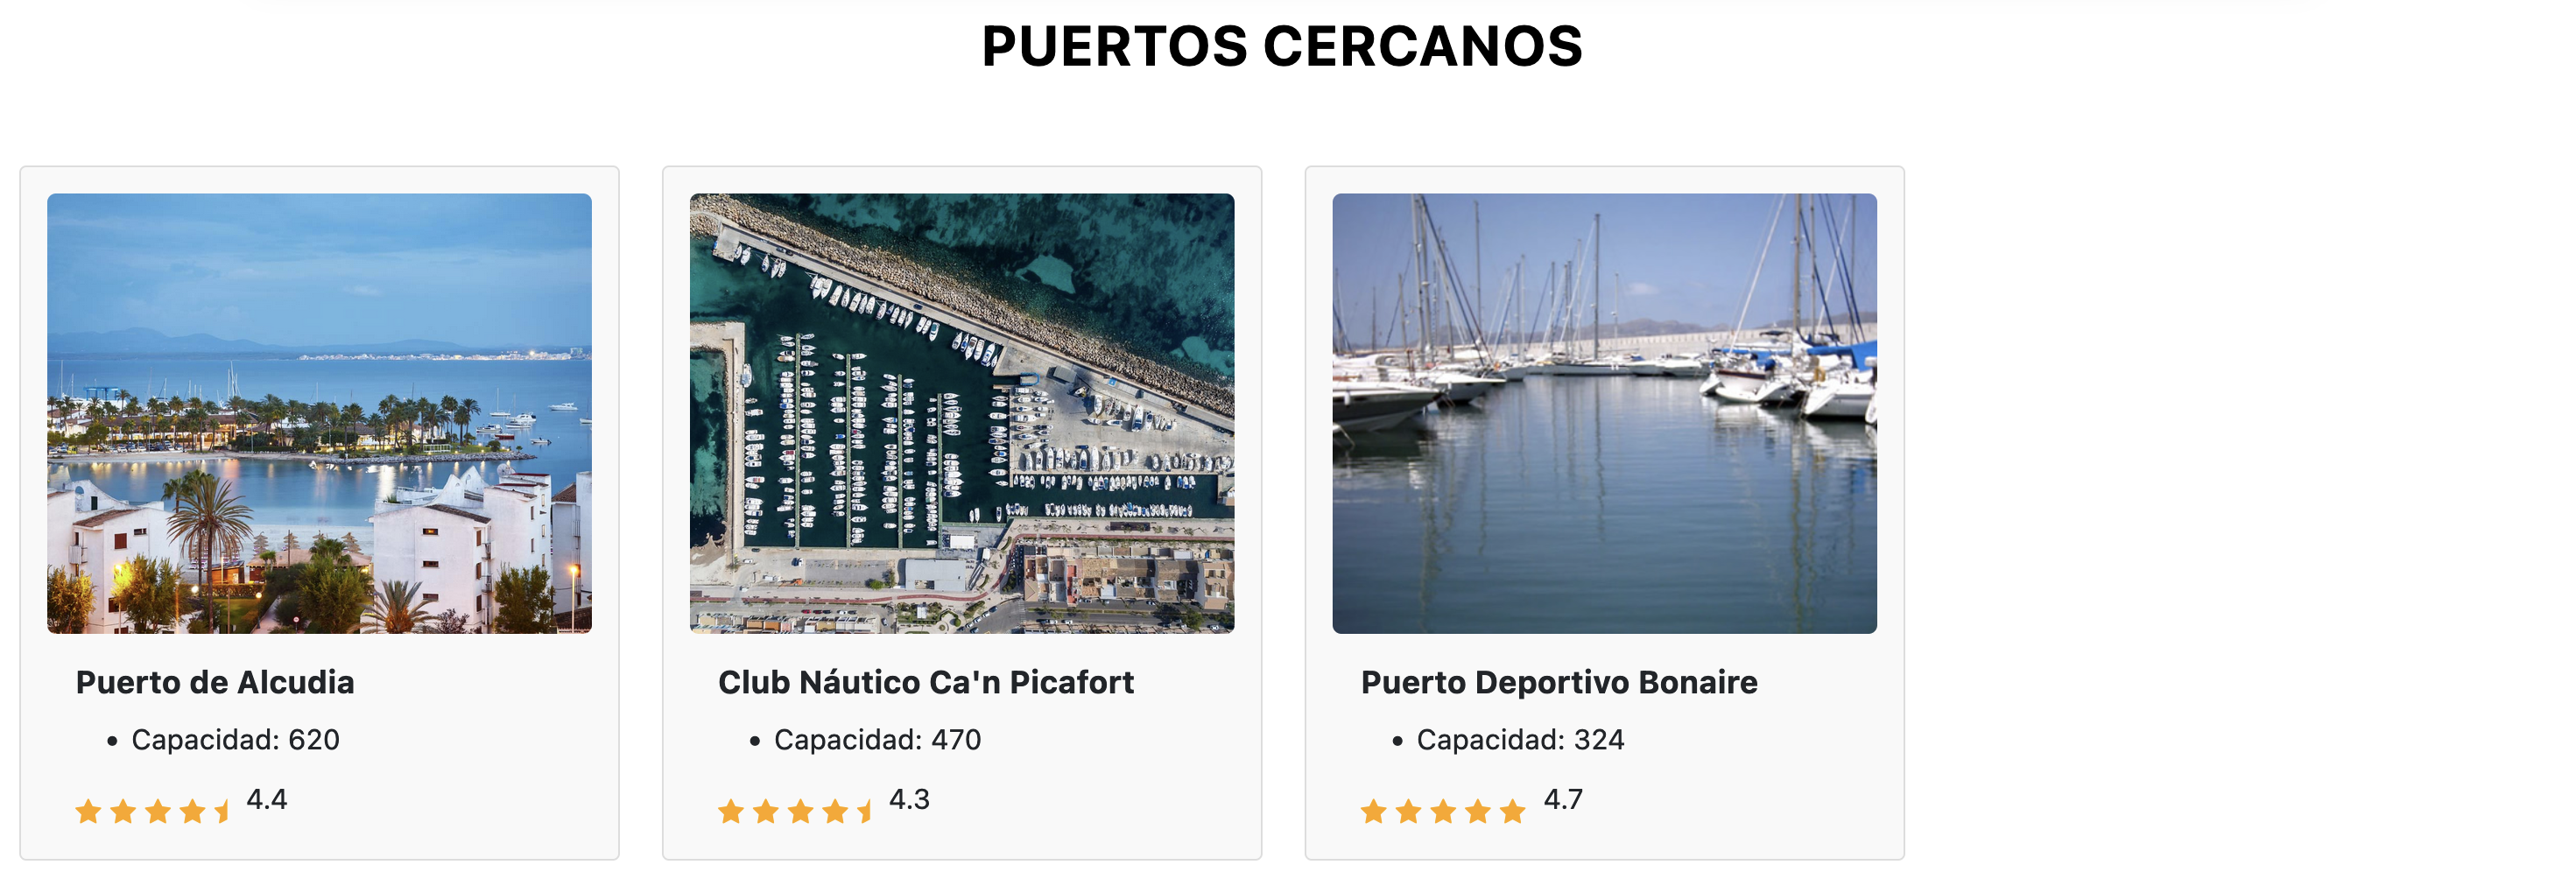
\includegraphics[width=0.7\textwidth]{images/puertosCercanos.png}
        \caption{Como se muestran los puertos cercanos}
    \end{figure}
\end{itemize}

\subsection{Página de Contacto}
Para finalizar con las funcionalidades de la web-app, llegamos a la pagia donde el usuario puede contactar con nosotros, los creadores para aportar sugerencias o resolver dudas que le puedan surgir durante la utilización de la web-app. Lo que nos encontramos en la sección llamada \textit{Sobre Nosotros} es lo siguiente:

\begin{itemize}
    \item \textbf{Video}: video explicativo donde nos presentamos al usuario como creadores de la pagina.\textbf{Falta grabar el video}
    \item \textbf{Sección de Contacto}: en esta sección, el usuario tiene la posibilidad de enviarnos un correo, pudiendo apuntar el tipo de asunto del correo, su nombre, su correo y el mensaje que nos quiere hacer llegar. En caso que el usuario quiera satisfacer sus inquietudes sobre algo relacionado con la web-app, podrá hacerlo mediante este formulario.
    \begin{figure}[ht]
        \centering
        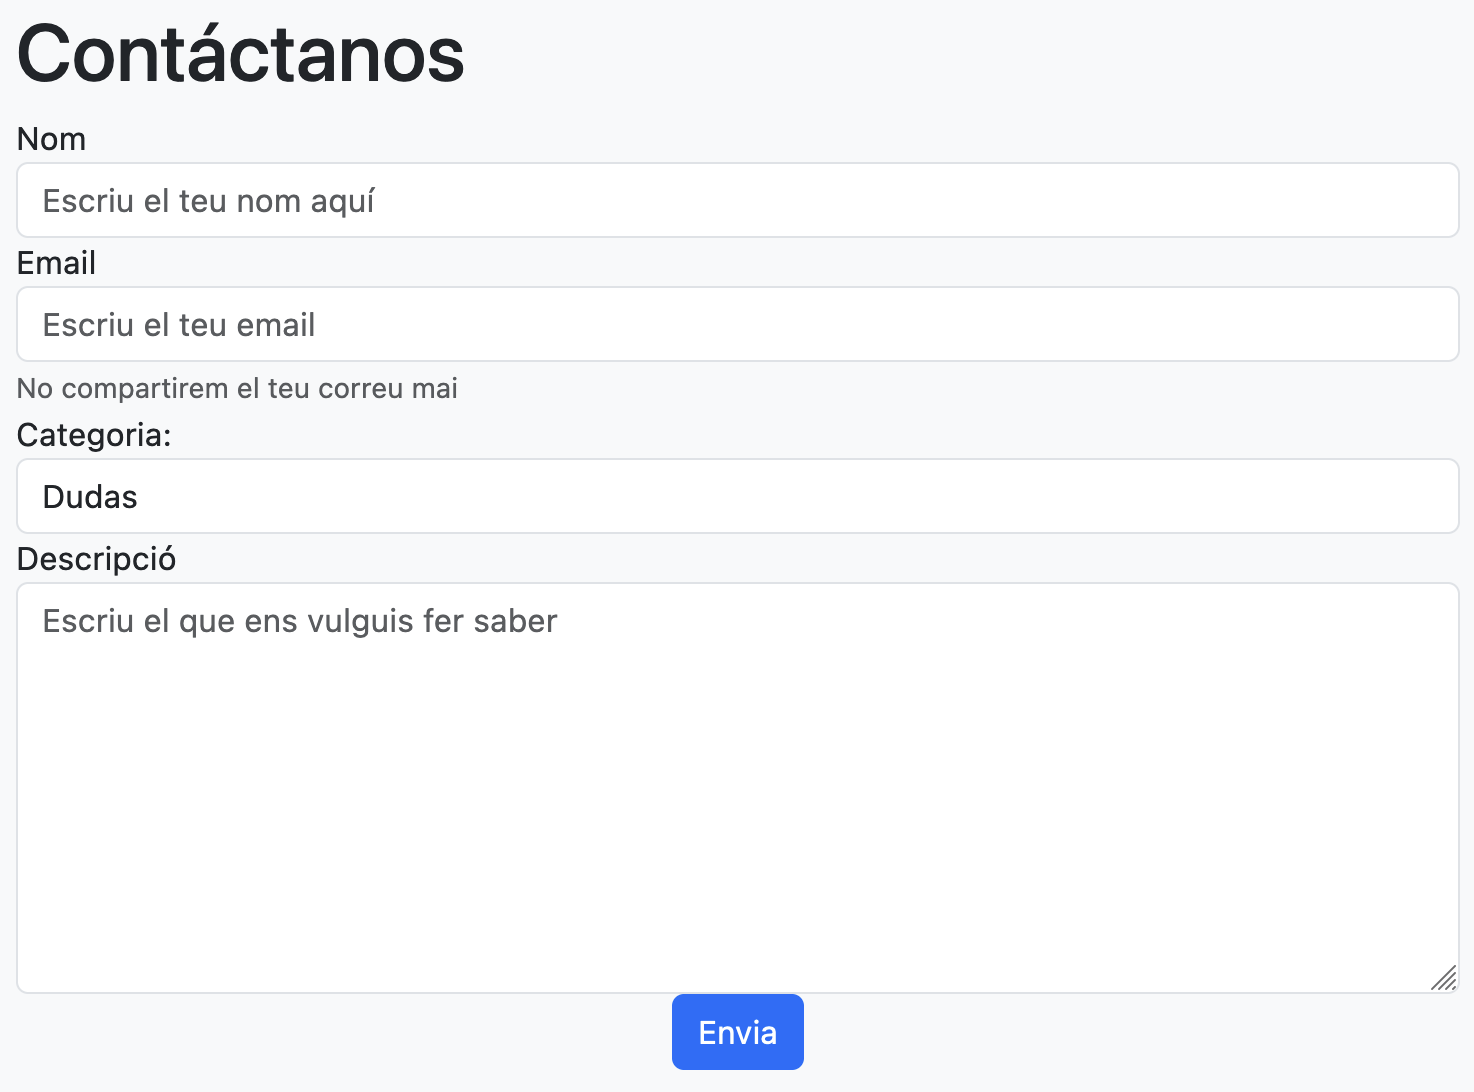
\includegraphics[width=0.5\textwidth]{images/contacto.png}
        \caption{Sección en la qual el usuario nos puede contactar}
    \end{figure}
\end{itemize}
\newpage
\section{Herramientas y Librerias}
Una vez se han explicado todas las funcionalidades que el usuario puede realizar en nuestra web-app, pasaremos a la explicación técnica de como se han implementado todas esas funcionalidades. Iremos revisando una por una las componentes de todas las páginas de la web-app y explicando que herramientas y librerías se han usado para su desarrollo.
\subsection{index.html}
El archivo \texttt{index.html} contiene el código HTML de la \textit{homepage}. El contenido funcional de esta parte de la web-app ya se ha explicado a nivel de usuario, en esta sección se describirá como se han desarrollado esas funcionalidades a nivel técnico.

\subsubsection{Barra de Navegación}

\noindent Para la creación de la barra de navegación, se ha usado el framework \href{https://getbootstrap.com/}{Bootstrap}. Primero, hemos definido un objeto de la clase \texttt{container-fluid} el cual contendrá todo lo referente a la barra de navegación. Por otro lado, hemos añadido atributos a este contenedor para que el aspecto final de la barra de navegación sea el deseado:
\begin{itemize}
    \item \texttt{px-0}: elimina los márgenes horizontales (padding) del elemento, lo que significa que el contenido del elemento se extiende hasta los bordes laterales del contenedor.
    \item \texttt{d-flex}: define el elemento como un contenedor flexible, lo que significa que sus elementos hijos se pueden ajustar dinámicamente para adaptarse a diferentes tamaños de pantalla.
    \item \texttt{align-items-center}: alinea verticalmente los elementos hijos del contenedor, centrándolos en el eje vertical.
    \item \texttt{fixed-top}: fija el elemento en la parte superior de la pantalla, de modo que permanece en su posición incluso cuando el usuario se desplaza hacia abajo en la página.
\end{itemize}
Una vez sabemos como hemos definido el contendor, vamos con los elementos que se encuentran dentro de este. El principal elemento es un objeto de la clase \texttt{navbar navbar-expand-lg}. Esta, se utiliza para crear una barra de navegación responsiva en un sitio web (esto último es lo que indica el \texttt{expand-lg}). Dentro de esta, encontramos ya los botones que contienen la barra de navegación:
\begin{itemize}
    \item \textbf{Logo}: se ha realizado mediante la clase \texttt{navbar-brand}, perteneciente a Bootstrap. Dentro de este se encuentra la imagen del mismo.
    \item \textbf{Nombre de la página}: el nombre de \textit{Puertos Mallorca} contenido en la barra de navegación, se encuentra dentro del objeto del logo. Este es otro objeto de la clase \texttt{navbar-brand}.
    \item \textbf{Botón de navegación}: este botón solo aparece en caso de que la pantalla donde se muestra la web-app no sea lo suficientemente grande como para mostrar todos los botones de la barra de navegación. En caso de suceder esto, aparecerá un botón con el cual podremos acceder a los botones que explicamos a continuación. Esto se ha hecho gracias a la clase \texttt{navbar-toggler} de Bootstrap. referenciando al objeto al que influye con el parámetro \texttt{aria-controls}. Mediante este, indicamos que el objeto con \texttt{id = navbarSupportedContent} se le aplicará la contracción de los botones cuando la pantalla no se alo suficientemente grande.
    \item \textbf{Botones de funcionalidades}: los botones de \textit{Ver Puertos} y \textit{Contacto} son objetos del tipo \texttt{nav-item} (items de una barra de navegación) de boostrap y están contenidos dentro de un objeto \texttt{collapse navbar-collapse}. Este objeto permite la contracción de los botones que hemos explicado en el apartado anterior.
\end{itemize}
\newpage
A continuació se muestra el codigo referente a la barra de navegación:
\begin{minted}[bgcolor=mybgcolor, escapeinside=||]{html}
<div class="container-fluid px-0 d-flex align-items-center fixed-top">
    <!-- Navegation bar -->
    <nav class="navbar navbar-expand-lg" data-bs-theme="light" id="nvar">
        <div class="container-fluid">
            <!-- LOGO -->
            <a class="navbar-brand ms-3" href="index.html" id="contenidorLogo">
                <img src="ancla.svg" alt="Logo" width="27" height="43" 
                class="d-inline-block align-text-bottom" />
                <a class="navbar-brand mb-0 h1" href="#index.html">
                    |\textcolor{white}{Puertos mallorca}|</a>
            </a>
            <!-- END LOGO -->
            <button class="navbar-toggler" type="bsutton" 
            data-bs-toggle="collapse" data-bs-target="#navbarSupportedContent" 
            aria-controls="navbarSupportedContent"
            aria-expanded="false" aria-label="Toggle navigation">
                <span class="navbar-toggler-icon"></span>
            </button>
            <div class="collapse navbar-collapse" id="navbarSupportedContent">
                <ul class="navbar-nav ms-auto mb-2 mb-lg-0">
                    <li class="nav-item me-3">
                        <a class="nav-link" href="#contenedorMapa">
                            |\textcolor{white}{Ver puertos}|</a>
                    </li>
                    <li class="nav-item me-3">
                        <a class="nav-link" href="sobreNosotros.html">
                        |\textcolor{white}{Sobre Nosotros}|</a>
                    </li>
                </ul>
            </div>
        </div>
    </nav>
    <!-- END Navegation bar -->
</div>
\end{minted}

\subsubsection{Carousel}
El deslizable con fotografias de los puertos, se ha realizado cogiendo como base la tercera de las \href{https://getbootstrap.com/docs/5.3/components/carousel/}{plantillas} que proporciona la página de boostrap para hacer estos carousels. Partiendo de esa base, nosostros hemos añadido las captions y la flecha que permite al ususario ir más abajo de la página. Las captions se crean con ojectos de la clase \texttt{carousel-caption} y los botones para ir más abajo de la página, son objetos de la classe \texttt{btn btn-down} de boostrap. Estos nos permiten crear un boton con forma de flecha como la que aparece en la web-app y mediante un \texttt{href} en su interior, linkeado con la parte inroductoria de la página, hacemos que cuando cliquemos encima de este nos lleve más abajo. A continuación se muestra el código referente al carrousel de nuestra web-app:
\begin{minted}[bgcolor=mybgcolor, escapeinside=||]{html}
<!-- CARROUSEL-->
<div id="carouselInit" class="carousel slide mt-0" data-bs-ride="carouselInit">
    <div class="carousel-indicators">
        <button type="button" data-bs-target="#carouselInit" data-bs-slide-to="0"
         class="active" aria-current="true" aria-label="Slide 1"></button>
        <button type="button" data-bs-target="#carouselInit" data-bs-slide-to="1" 
        aria-label="Slide 2"></button>
        <button type="button" data-bs-target="#carouselInit" data-bs-slide-to="2" 
        aria-label="Slide 3"></button>
    </div>
    <div class="carousel-inner">
        <div class="carousel-item active">
            <img src="portI5.jpg" class="d-block w-100" alt="...">
            <div class="carousel-caption" id="carousel-text1">
                <h1>|\textcolor{white}{Bienvenido a Puertos Mallorca!}|</h1>
                <p>|\textcolor{white}{Una guia completa de todos los puertos de la isla}|</p>
                <button id="btnDown1" type="button" class="btn btn-down">
                    <a href="#intro" id="link1">
                        <i class="fas fa-chevron-down"></i></a></button>
            </div>
        </div>
        <div class="carousel-item">
            <img src="portI1.jpg" class="d-block w-100" alt="...">
            <div class="carousel-caption" id="carousel-text2">
                <h1>|\textcolor{white}{Descubre todo lo que no sabias!}|</h1>
                <p>|\textcolor{white}{Navega entre los puertos mejor valorados de la isla}|</p>
                <button id="btnDown2" type="button" class="btn btn-down">
                    <a href="#intro" id="link2">
                        <i class="fas fa-chevron-down"></i></a></button>
            </div>
        </div>
        <div class="carousel-item">
            <img src="portI4.jpg" class="d-block w-100" alt="...">
            <div class="carousel-caption" id="carousel-text3">
                <h1>|\textcolor{white}{Crea tu plan de navegación!}|</h1>
                <p>|\textcolor{white}{Podras crear tu plan para navegar por las costas}| 
                |\textcolor{white}{mallorquinas}|</p>
                <button id="btnDown3" type="button" class="btn btn-down">
                    <a href="#intro" id="link3">
                        <i class="fas fa-chevron-down"></i></a></button>
            </div>
        </div>
    </div>
    <button class="carousel-control-prev" type="button" 
    data-bs-target="#carouselInit" data-bs-slide="prev">
        <span class="carousel-control-prev-icon" 
        aria-hidden="true"></span>
        <span class="visually-hidden">|\textcolor{white}{Previous}|</span>
    </button>
    <button class="carousel-control-next" type="button" 
    data-bs-target="#carouselInit" data-bs-slide="next">
        <span class="carousel-control-next-icon" 
        aria-hidden="true"></span>
        <span class="visually-hidden">|\textcolor{white}{Next}|</span>
    </button>
</div>
<!-- END CARROUSEL-->
\end{minted}

\subsubsection{Sección introductoria}
Este apartado contiene dos secciones principales: una sección de introducción con una imagen y un texto descriptivo, y una sección de tres columnas con información destacada sobre los puertos de Mallorca.\\

\noindent En la sección de introducción, hemos hecho un contenedor de HTML div con la clase \texttt{site-section} y un identificador \texttt{intro}. Dentro de este contenedor, hay otro contenedor de \texttt{div} con la clase \textit{container} y un contenedor de fila de div con la clase \texttt{row}. Esta fila contiene dos columnas de div con las clases \texttt{col-md-6} de Bootstrap. En la primera columna, hay una imagen con la clase \texttt{img-fluid}. En la segunda columna, hay un título con la clase \texttt{text-black} y un subtítulo con la clase \texttt{text-primary}.\\

\noindent En la sección de tres columnas, encontramos un contenedor de div con la clase \texttt{py-5}, un contenedor de div con la clase \texttt{container} y un contenedor de fila de div con la clase \texttt{row}. Dentro de esta fila, hay tres columnas de div con las clases \texttt{col-md-6 col-lg-4} también de boostrap. Cada columna contiene un contenedor de div con la clase "puertosIncreibles" (clase que luego usamos para referencial algunos objetos en css) que contiene un icono en un contenedor de \textit{span} con la clase \textit{circulo} y un título de ancla con la clase \texttt{tituloIntroduccion}. En resumen, esta sección presenta una breve introducción a la página y destaca tres características principales de la web relacionadas con los puertos de Mallorca.\\

\noindent Para la creación de esta sección introductoria, nos hemos inspirado en una sección similar que encontramos en \href{https://themewagon.github.io/waterboat/}{esta plantilla}.

\begin{minted}[bgcolor=mybgcolor, escapeinside=||]{html}
<!-- Sección introductoria a la página -->
<div class="site-section " id="intro">
    <div class="container">
        <div class="row">
            <div class="col-md-6">
                <img src="portI6.jpg" alt="Image" class="img-fluid">
            </div>
            <div class="col-md-6">
                <span class="text-serif text-primary">|\textcolor{white}{Sobre nosotros}|</span>
                <h3 class="text-black">|\textcolor{white}{Bienvenido a nuestra pagina}|</h3>
                <p class="texto">|\textcolor{white}{En esta pagina podrás obtener toda la}|
                    |\textcolor{white}{información sobre los puertos de mallorca. Información}| 
                    |\textcolor{white}{de contacto, localización, valoraciones, numero}|
                    |\textcolor{white}{de amarres...}|</p>
                <p class="texto">|\textcolor{white}{Además, te damos la posibilidad de crear tu hoja}| 
                    |\textcolor{white}{de navegación para poder navegar por las aguas mallorquinas }|
                    |\textcolor{white}{de la forma en que más te guste.}|</p>
            </div>
        </div>
    </div>

    <div class="py-5">
        <div class="container">
            <div class="row">
                <div class="col-md-6 col-lg-4">
                    <div class="puertosIncreibles">
                        <span class="circulo">
                            <i class="fas fa-ship"></i>
                        </span>

                        <h3><a class="tituloIntroduccion" href="#contenedorMapa">
                            |\textcolor{white}{Puertos increibles}|</a></h3>

                        <p class="texto">|\textcolor{white}{Tenemos registrados los principales}|
                        |\textcolor{white}{puertos de mallorca y subiendo!}|</p>
                    </div>
                </div>
                <div class="col-md-6 col-lg-4">
                    <div class="puertosIncreibles">
                        <span class="circulo">
                            <i class="fas fa-anchor"></i>
                        </span>
                        <h3><a class="tituloIntroduccion" href="#contenedorMapa">
                            |\textcolor{white}{Navega}|</a></h3>
                        <p class="texto">|\textcolor{white}{Crear tu propio plan de navegación}|
                            |\textcolor{white}{para disfrutar al máximo de tus calas y lugares}|
                            |\textcolor{white}{de interés favoritos de mallorca}|</p>
                    </div>
                </div>
                <div class="col-md-6 col-lg-4">
                    <div class="puertosIncreibles">
                        <span class="circulo">
                            <i class="fas fa-thumbs-up"></i>
                        </span>
                        <h3><a class="tituloIntroduccion" href="#contenedorMapa">
                            |\textcolor{white}{Garantizado}|</a></h3>
                        <p class="texto">|\textcolor{white}{Con nuestro plan seguro que que acabas}| 
                            |\textcolor{white}{ descubriendo más de lo que pensabas!}|</p>
                    </div>
                </div>
            </div>
        </div>
    </div>
</div>
<!-- END Sección introductoria a la página -->
\end{minted}

\subsubsection{Mapa de puertos}
Para la creación del mapa, hemos usado la API que proporciona Google de su servicio Google Maps. Con esta, podemos mostrar un mapa de google maps interactivo, ademas de los marcadores de los puertos que tenemos registrados en la pagina.\\

\noindent El mapa se encuentra contenido dentro de un objeto de la clase \texttt{container-fluid} de Bootstrap. Dentro de este, hemos añadido el \texttt{div} correspondiente al mapa, el cual le hemos añadido el identificador \texttt{map}. En cuanto al HTML, esto sería todo lo que necesitamos para crear el mapa. Siguiendo la documentación que proporciona Google sobre como crear los mapas, hemos implementado el fichero de JavaScript adjuntado en el proyecto llamado \texttt{mapa.js}. Este contiene las instrucciones necesarias para la creación del mapa en la web-app (Estas instrucciones concretas se explicaran más adelante en el documento, así como las instrucciones que usamos para la lectura y obtención de la información del fichero json).\\

\noindent El código html con el que generamos el mapa interactivo és el siguiente:s 
\begin{minted}[bgcolor=mybgcolor, escapeinside=||]{html}
<!-- MAP-->
<div class="container-fluid" id="contenedorMapa">
    <div class="container" id="titolMapa">
        <h2 class="text-center">|\textcolor{white}{Puertos de Mallorca}|</h2>
    </div>
    <div id="map"></div>
</div>
<!--END MAP-->
\end{minted}

\subsubsection{Barra de filtros}
Para la barra de filtros y ordenación, también hemos usado el framework Bootstrap. Por tanto, todas las clases que se usan para los elementos de la barra de filtros son pertenecientes a este.\\

\noindent Toda la barra de filtros está contenida dentro de un elemento de la clase \texttt{container-fluid} para hacer que el contenedor ocupe todo el ancho de la pantalla. Dentro de este contenedor, hay un elemento \texttt{row} con la clase \texttt{filterSearch} y \texttt{align-items-center}, lo que indica que se trata de una fila que contiene elementos centrados verticalmente. Además, hemos utilizado la clase \texttt{py-2} para agregar un espacio vertical a la fila. Dentro de la fila, hay cuatro columnas definidas usando la clase \texttt{col-xs-12 col-sm-6 col-md-3}. Estas columnas son para los elementos de búsqueda por nombre, valoración, capacidad y ordenar por. Dentro de cada columna, se utiliza la clase \texttt{input-group} para agregar estilos a los elementos de entrada de texto y select. Cada uno de estos elementos tiene una etiqueta de texto que describe la entrada que se espera.\\

\noindent El botón de búsqueda está dentro de una columna de 12 columnas y utiliza la clase \texttt{d-flex justify-content-center} para centrarlo horizontalmente. Se le da un identificador \texttt{botoCerca} (que usaremos posteriormente en los scripts de JavaScript) y se le asigna la clase \texttt{btn btn-primary mt-3} para darle un estilo de botón. Además, se utiliza la función \texttt{PortSearch()} \textbf{(actualmente no está desarrollada esta función, pero será la encargada de que se muestren unos puertos u otros en la siguiente sección de la web-app)} cuando se hace clic en el botón.

\subsubsection{Cards de puertos}
Justo debajo de la barra de filtros, encontramos los puertos que podemos filtrar i ordenar mediante esta. Esta sección se encuentra encapsulada en un \texttt{container-fluid} de Bootstrap, de los cuales ya hemos hablado en esta documentación. Dentro de este contenedor, encontramos varias filas de objetos de la clase \texttt{card}. Las filas las definimos mediante la clase \texttt{row equal-width} y las columnas de estas filas con la clase \texttt{col-md-3}.\\

\noindent Por lo que respecta a los recuadros de los puertos, el framework de Bootstrap tiene una clase llamada \href{https://getbootstrap.com/docs/5.3/components/card/}{Card}, con la cual puedes crear recuadros con una foto y una pequeña sección de texto. Este tipo de objetos son los que hemos elegido para mostrar una previsualización de los puertos registrados en la página.\\

\noindent La estructura que siguen todas las \texttt{cards} es la siguiente:
\begin{itemize}
    \item El primer elemento es una etiqueta \texttt{a} que envuelve una imagen (\texttt{img}) y que sirve como enlace a la página del puerto al que pertenezca la \texttt{card}. Mediante este enlace, el usuario podrá navegar y ver la información de diferentes puertos.
    \item El segundo elemento es un \texttt{div} con la clase \texttt{card-body} que contiene el contenido principal de la card. Dentro de este, mostraremos la información textual del puerto (nombre, capacidad y valoración).
    \item Dentro del div con la clase \texttt{card-body}, hay un elemento h5 con la clase \texttt{card-title} que muestra el título de la card (en este caso será el nombre del puerto).
    \item También hay una lista no ordenada (\texttt{ul}) con un solo elemento (\texttt{li}) que muestra la capacidad del puerto.
    \item Finalmente, hay un \texttt{div} con la clase rating que contiene estrellas de valoración de la clase \texttt{fa fa-star} y un párrafo (\texttt{p}) que muestra la valoración promedio del puerto.
\end{itemize}

Todos estos tipos de objetos de boostrap, los generamos mediante el fichero JavaScript llamado \texttt{port.js}. El contenido de este se mostrará más adelante, pero básicamente generamos el código html del \texttt{div} con nombre \texttt{contenedorPrepuertos}medida que vamos leyendo el contenido del fichero json. De esta forma, solo creeamos los objetos de \texttt{boostrap} necesarios segun el número de puertos que haya en el fichero. Se crearan los objetos html de forma dinámica.\\

\noindent El código html con el que generamos la sección de \texttt{cards} de puertos es el siguinte:
\begin{minted}[bgcolor=mybgcolor, escapeinside=||]{html}
<!--DISPLAY ALL PORTS-->
<div class="container-fluid" id="contenedorPrePuertos">
    <!-- FILA PUERTOS-->
</div>
<!-- END DISPLAY ALL PORTS-->
\end{minted}

\subsubsection{Footer}
Finalmente, en la \textit{homepage} encontramos el footer. Esta sección comienza con una etiqueta \texttt{<footer>} que tiene una clase \texttt{bg-dark text-light py-5}, lo que significa que el fondo del pie de página será oscuro y el texto será claro. Además, el padding superior e inferior de la sección será de 5 píxeles.\\

\noindent Dentro del pie de página hay un contenedor de la clase \texttt{container} que contiene una fila (\texttt{row}) con cuatro columnas (\texttt{col-md-3 mb-4 mb-md-0}), cada una con información de un miembro del equipo.\\

\noindent Cada columna comienza con un encabezado (\texttt{fw-bold mb-2}) que muestra el nombre del miembro del equipo y luego se muestran tres iconos que representan los enlaces a los perfiles de cada miembro en Github, Linkedin e Instagram respectivamente. Los enlaces se abren en una nueva ventana (\texttt{target="\_blank"}) y no se les permite la seguridad adicional de referencias (\texttt{rel="noopener noreferrer"}).\\

\noindent El código html que general nuestro footer és el siguiente:
\begin{minted}[bgcolor=mybgcolor, escapeinside=||]{html}
<!-- Footer -->
<footer class="bg-dark text-light py-5">
    <div class="container">
        <div class="row">
            <div class="col-md-3 mb-4 mb-md-0">
                <h4 class="fw-bold mb-2">|\textcolor{white}{Joan Balaguer}|</h4>
                <a href="https://github.com/Joan13the13the13" target="_blank" 
                rel="noopener noreferrer" class="text-light">
                <i class="fab fa-github"></i></a>
    <a href="https://www.linkedin.com/in/joan-balaguer-llagostera-50839a269/" 
    target="_blank" rel="noopener noreferrer" class="text-light">
    <i class="fab fa-linkedin"></i></a>
            <a href="https://www.instagram.com/joan_balaguer/" 
            target="_blank" rel="noopener noreferrer"
            class="text-light"><i class="fab fa-instagram"></i></a>
            </div>
            <div class="col-md-3 mb-4 mb-md-0">
                <h4 class="fw-bold mb-2">|\textcolor{white}{Diego Bermejo}|</h4>
                <ul class="list-unstyled">
                    <a href="https://github.com/diegofes18" target="_blank" 
                    rel="noopener noreferrer" class="text-light">
                    <i class="fab fa-github"></i></a>
    <a href="https://www.linkedin.com/in/diego-bermejo-caba%C3%B1as-742393216/"
        target="_blank" rel="noopener noreferrer" class="text-light">
        <i class="fab fa-linkedin"></i></a>
            <a href="https://www.instagram.com/diegofes_18/" target="_blank"
            rel="noopener noreferrer" class="text-light">
            <i class="fab fa-instagram"></i></a>
            </div>
            <div class="col-md-3 mb-4 mb-md-0">
                <h4 class="fw-bold mb-2">|\textcolor{white}{Jaume Adrover}|</h4>
                <a href="https://github.com/jaaumeadrover" target="_blank" 
                rel="noopener noreferrer" class="text-light">
                <i class="fab fa-github"></i></a>
    <a href="https://www.linkedin.com/in/jaume-adrover-fern%C3%A1ndez-1943411b3/" 
    target="_blank" rel="noopener noreferrer" class="text-light">
    <i class="fab fa-linkedin"></i></a>
            <a href="https://www.instagram.com/jaaumeadrover/" 
            target="_blank" rel="noopener noreferrer" class="text-light">
            <i class="fab fa-instagram"></i></a>
                </ul>
            </div>
            <div class="col-md-3 mb-4 mb-md-0">
                <h4 class="fw-bold mb-2">|\textcolor{white}{Marc Cañellas}|</h4>
                <a href="https://github.com/MarcCanellasG" target="_blank" 
                rel="noopener noreferrer" class="text-light">
                <i class="fab fa-github"></i></a>
    <a href="https://www.linkedin.com/in/marc-ca%C3%B1ellas-74a629255/"
    target="_blank" rel="noopener noreferrer" class="text-light">
    <i class="fab fa-linkedin"></i></a>
            <a href="https://www.instagram.com/maarccanellas/" target="_blank"
            rel="noopener noreferrer" class="text-light">
            <i class="fab fa-instagram"></i></a>
                </ul>
            </div>
        </div>
    </div>
</footer>
<!--END FOOTER-->
\end{minted}

\subsection{puerto.html}
En este fichero HTML está contenido las estructuras para poder mostrar al usuario la información sobre un puerto en concreto. En las explicaciones siguientes, se obvian la barra de navegación y el footer (ya explicados en la \textit{homepage}). Cabe mencionar que en este fichero la mayoria de atributos que ahora mostraremos no tienen su contenido escrito como tal. Lo que tienen es su estructura html con un \texttt{<span></span>} que tiene un identificador. Mediante este id, en el fichero \texttt{port.js} le insertamos el contenido cuando leemos la información sobre el puerto correspondiente (en el apartado de archivos JavaScript mostraremos los detalles de la implementación que hace esto posible).

\subsubsection{Nombre del puerto}
El nombre del puerto simplemente de trata de un contenedor con un \texttt{h1} que muestra bien en grande como se llama el puerto seleccionado. Además, mediante \textit{CSS} se ha añadido una imagen de fondo para dar un ambiente más marino. Dentro del elemento \texttt{h1} se encuentra el elemento \texttt{span} ya mencionado.\\

\noindent El código que lo genera el es siguiente:

\begin{minted}[bgcolor=mybgcolor, escapeinside=||]{html}
<!-- Nombre del Puerto -->
<div class="titulo" id="titulo">
  <h1><span id="port-name"></span></h1>
</div>
<!-- END Nombre del Puerto-->    
\end{minted}

\subsubsection{Descripción y Video}
En esta sección de la página, se muestra la descripción del puerto seleccionado, además de un video que lo muestra. Ambas cosas son atributos que obtenemos del fichero JSON de puertos. El como leemos e insertamos estos atributos en la pagina se explicará en el apartado de ficheros JavaScript.\\

\noindent Los dos atributos se encuentran en un objeto \texttt{container-fluid} y dentro de este mostramos una fila con dos columnas. Cada una de ellas es uno de los atributos. La descripción está contenida en una columna de la clase \texttt{col-md-8 col-lg-6} y el video en una columna de clase \texttt{col-md-4 col-lg-6 mb-4 align-self-center}. El video se encuentra en un \texttt{div} de clase \texttt{embed-responsive embed-responsive-16by9 custom-embed-responsive}, que nos permite poner un video de YouTube justo al lado de la descripción del puerto, de forma que este se pueda reproducir sin necesidad de abrir una pestaña nueva con el link del video.

\subsubsection{Características i Tiempo}
En esta secció, se mustran todas las otras características del puerto junto con el tiempo que hace en este. Las características son todas atributos de dentro del json mientras que el tiempo en ese puerto lo podemos obtener gracias a las coordenadas del puerto (que son dos atributos del puerto en el json).\\ 

\noindent\texttt{<div id="car-tiempo" class="container-fluid">}: Este es un contenedor \texttt{<div>} con un ID \texttt{car-tiempo} y la clase \texttt{container-fluid}. La clase \texttt{container-fluid} se utiliza en Bootstrap para crear un contenedor que ocupa todo el ancho de la pantalla, como ya se ha mencionado en ocasiones anteriores en el documento.\\

\noindent\texttt{<div class="row">}: con esto, creamos una fila dentro del contenedor. En Bootstrap, las filas se utilizan para organizar y alinear los elementos en una cuadrícula.\\

\noindent\texttt{<div class="col-md-8 mb-4" data-aos="fade-right" aos-duration="1000" aos-delay="1500">}: Este \texttt{<div>} crea una columna dentro de la fila. La clase \texttt{col-md-8} indica que esta columna ocupará 8 columnas de ancho en pantallas medianas y más grandes. La clase \texttt{mb-4} se utiliza para agregar un margen inferior de tamaño medio. Los atributos de datos \texttt{data-aos}, \texttt{aos-duration} y \texttt{aos-delay} se utilizan para animar la aparición de la columna utilizando la biblioteca AOS (Animate On Scroll).\\

\noindent\texttt{<table class="table">}: Esto crea una tabla con la clase \texttt{table}. En Bootstrap, la clase \texttt{table} se utiliza para aplicar estilos predefinidos a las tablas. Dentro de la tabla, hay varias filas (\texttt{<tr>}) que contienen datos sobre las características de un puerto náutico, como la capacidad de barcos, si permite fumar, horarios, dirección, información de contacto, etc. Cada fila contiene dos celdas (\texttt{<td>}): una para el ícono y el título, y otra para el valor correspondiente al atributo del puerto. Los valores se representan dentro de elementos \texttt{<span>} con IDs específicos. Estos IDs son los que usaremos para insertar el contenido de estos mediante JavaScript de forma dinámica.\\

\noindent Después de la columna anterior, hay otra columna \texttt{<div>} con la clase \texttt{col-md-4 mb-4}. Esta columna ocupará 4 columnas de ancho en pantallas medianas y más grandes. Dentro de esta columna, hay un contenedor \texttt{<div>} con el ID \texttt{tiempo} que alberga información sobre el clima del puerto. Hay tres bloques (\texttt{<div class="box">}) que muestran información como la temperatura, humedad y velocidad del viento. Estas características se pueden mostrar gracias a que usamos la API OpenWeatherAPI. El como la usuamos, lo mostraremos en el apartado de APIs. Cada valor de la climatología se representa dentro de elementos \texttt{<span>} con IDs específicos. Estos IDs son los que usaremos para insertar el contenido de estos mediante JavaScript de forma dinámica.\\

\noindent El código html que usuamos para mostrar la tabla de características y el tiempo es el siguiente:
\begin{minted}[bgcolor=mybgcolor, escapeinside=||]{html}
<!-- Caracteristicas del Puerto -->
<div id="desc-video" class="container-fluid">
<div class="row">
    <div class="col-md-8 col-lg-6">
    <!-- Puerto Náutico Descripción -->
    <div class="mb-3 text">
        <p><span id="port-descr"></span></p>
    </div>
    </div>
    <div class="col-md-4 col-lg-6 mb-4 align-self-center">
    <div class="embed-responsive embed-responsive-16by9 custom-embed-responsive">
        <div id="player"></div>
    </div>
    </div>
</div>
</div>

<div id="car-tiempo" class="container-fluid">
<!-- Puerto Náutico Características -->
<div class="row">
    <div class="col-md-8 mb-4" data-aos="fade-right" aos-duration="1000" 
    aos-delay="1500">
    <table class="table">
        <tbody>
        <tr>
            <td>
            <i class="fas fa-ship"></i>
            <strong>|\textcolor{white}{Capacidad de Barcos:}|</strong>
            </td>
            <td><span id="port-capacidad"></span></td>
        </tr>
        <tr>
            <td>
            <i class="fas fa-smoking-ban"></i>
            <strong>|\textcolor{white}{Permite Fumar:}|</strong>
            </td>
            <td><span id="port-smoke"></span></td>
        </tr>
        <tr>
            <td>
            <i class="far fa-clock"></i>
            <strong>|\textcolor{white}{Horario entre semana:}|</strong>
            </td>
            <td><span id="port-horaES"></span></td>
        </tr>
        <tr>
            <td>
            <i class="far fa-clock"></i>
            <strong>|\textcolor{white}{Horario fin de semana:}|</strong>
            </td>
            <td><span id="port-horaFS"></span></td>
        </tr>
        <tr>
            <td>
            <i class="fas fa-map-marker-alt"></i>
            <strong>|\textcolor{white}{Calle:}|</strong>
            </td>
            <td><span id="port-calle"></span></td>
        </tr>
        <tr>
            <td>
            <i class="fas fa-map-marker-alt"></i>
            <strong>|\textcolor{white}{Localidad:}|</strong>
            </td>
            <td><span id="port-locality"></span></td>
        </tr>
        <tr>
            <td>
            <i class="fas fa-map-marker-alt"></i>
            <strong>|\textcolor{white}{Codigo Postal:}|</strong>
            </td>
            <td><span id="port-addressCode"></span></td>
        </tr>
        <tr>
            <td>
            <i class="fas fa-envelope"></i>
            <strong>|\textcolor{white}{Correo:}|</strong>
            </td>
            <td><span id="port-correo"></span></td>
        </tr>
        <tr>
            <td>
            <i class="fas fa-phone"></i>
            <strong>|\textcolor{white}{Telefono:}|</strong>
            </td>
            <td><span id="port-telephone"></span></td>
        </tr>
        <tr>
            <td>
            <i class="fas fa-star"></i>
            <strong>|\textcolor{white}{Valoración:}|</strong>
            </td>
            <td id="contenedorValoracio">
            </td>
        </tr>
        </tbody>
    </table>
    </div>
    <!-- Tiempo -->
    <div class="col-md-4 mb-4">
    <!-- Imagen -->
    <div id="tiempo" class="text-center" data-aos="fade-left" aos-duration="1000">
        <h3 id="tempCity"></h3>
    
        <div class="box">
        <img src="https://cdn-icons-png.flaticon.com/512/46/46303.png" 
        alt="Termómetro">
        <span id="temperature"></span>
        </div>
    
        <div class="box">
        <img src="https://cdn-icons-png.flaticon.com/512/1113/1113834.png" 
        alt="Humedo">
        <span id="humidity"></span>
        </div>
    
        <div class="box">
        <img src="https://cdn-icons-png.flaticon.com/512/1585/1585359.png" 
        alt="Viento">
        <span id="windSpeed"></span>
        </div>
    </div>
    </div>
</div>
<!-- END Caracteristicas del Puerto -->
\end{minted}

\subsubsection{Galería de Imagenes}
En esta sección se muestran las imagenes que se encuentran como atribuitos en el json de los puertos. Como la mayoria de elementos de este fichero, se generan mediante el fichero \texttt{port.js} y en el archivo html solo encontramos el esqueleto de donde se muestra la información que se genera de forma dinámica.\\

\noindent El código html simplemente consiste en en \texttt{container-fluid} ya mencionados anteriormente con un elemento de tipo \texttt{<h2>} en su interior.\\

\noindent El código html del que hablamos es el siguinte:
\begin{minted}[bgcolor=mybgcolor, escapeinside=||]{html}
<!-- Galeria de Imagenes -->
<div class="container-fluid" id="galeria-img">
  <h2>|\textcolor{white}{Galería de Imágenes}|</h2>
</div>
<!-- END Galeria de Imagenes -->
\end{minted}

\subsubsection{Lugares de interés cercanos}
En la sección de lugares de interes cercanos de un puerto encontramos dos partes principales:

\subsubsection{Restaurantes y Playas}
\textbf{FALTAN JSONs DE LOS DE PLAYAS Y RESTAURANTES}

\noindent El código html que nos aydua a generar el mapa con los restaurantes y playas cercanas es el siguiente:
\begin{minted}[bgcolor=mybgcolor, escapeinside=||]{html}
<!-- Restaurantes y Playas-->
<div class="container-fluid" id="contenedorMapa">
    <div class="container" id="titolMapa">
        <h2 class="text-center">|\textcolor{white}{Restaurantes y Playas cercanas}|</h2>
    </div>
    <div id="map"></div>
</div>
<!-- END Restaurantes y Playas--->
\end{minted}

\subsubsection{Puertos Cercanos}
En esta sección se muestran los puertos que se encuentran próximos al que el usuario ha seleccionado. La estructura html que usamos para mostrar la previsulización de un puerto es exactamente la misma que usamos para mosrarlos en la \textit{homepage}. Por tanto obviamos la explicación de las clases de \texttt{Bootstrap} ya que son idénticas. Eso si, la generación de los puertos que se tienen que mostrar es un poco diferente que en la \textit{homepage}. Esto se debe a que solo debemos mostrar un subconjunto de los puertos totales. Los detalles de como implementamos y generamos las \texttt{cards} que permiten mostrar los puertos cercanos, los explicaremos en el apartado de los archivos JavaScript cuando expliquemos el archivo \texttt{port.js}.\\

\noindent El código html que nos permite mostrar los puertos cercanos es el siguiente:
\begin{minted}[bgcolor=mybgcolor, escapeinside=||]{html}
<!-- Puertos ceranos -->
<div class="container" id="titolMapa">
    <h2 class="text-center">|\textcolor{white}{Puertos cercanos}|</h2>
</div>
<div class="container-fluid" id="contenedorPuertos"></div>
<!-- END Puertos ceranos-->
\end{minted}

\subsection{contact.html}
En este último fichero html encontramos la sección de contacto para el usuario ademas de información sobre los creadores de la página. En este último html, también obviaremos la explicación tanto de la barra de navegación como del footer (ya que se han explicado en apartados anteriores).\\

\noindent En cuanto a la parte principal del archivo, enconteramos que todo esta dentro de un objeto de la clase \texttt{container-fluid} que a su vez esta dentro de un objeto de tipo \texttt{site-section}. Esta última clase mencionada se utiliza comúnmente para definir una sección o bloque de contenido en una página web. Proporciona estilos y características visuales específicas para esa sección en particular. Estos estilos pueden incluir márgenes, rellenos, colores de fondo, bordes u otros atributos visuales que ayudan a estructurar y diseñar la página de contacto. Dentro de este \texttt{div} encontramos dos secciones:
\begin{itemize}
    \item \textbf{Video Presentación}: se trata de un video donde los creadores de la web-app nos mostramos y presentamos para darnos a conocer al usuario. Esta parte de la web ha sido generada usando las siguientes clases de \texttt{bootstrap}:
    \begin{itemize}
        \item \texttt{<div class="row">}: La clase \texttt{row} se utiliza en Bootstrap para crear una fila que contiene columnas. Se utiliza para establecer una estructura de cuadrícula en la que se pueden organizar los elementos de forma horizontal. Las columnas dentro de una fila deben sumar un total de 12 unidades para que se distribuyan correctamente en diferentes tamaños de pantalla.

        \item \texttt{<div class="col-md-6 col-sm-6">}: La clase \texttt{col-md-6} y \texttt{col-sm-6} se utilizan para crear una columna que ocupará la mitad del ancho total de la fila en pantallas medianas (\texttt{md}) y pequeñas (\texttt{sm}). Esto significa que la columna ocupará 6 unidades de ancho de las 12 unidades disponibles en la fila. Estas clases permiten que el diseño sea responsivo y se ajuste a diferentes tamaños de pantalla.
    \end{itemize}
    La explicación de las clases que usamos para mostrar el video en la web se explicaran mas adelante en el apartado de inclusión de media en nuestra web-app.
    \item \textbf{Formulario}: para poder mostrar un formulario para que el usuario nos pueda enviar sugerencias, reclamaciones o dudas, hemos usado la API \texttt{emailJS}. Por otra parte, para crear los campos donde el ususario tiene que insertar los datos són las siguientes:
    \begin{itemize}
        \item  \texttt{<div class="col-md-6 col-sm-6">}: Esta clase crea una columna que ocupará la mitad del ancho total de la fila en pantallas medianas y pequeñas. Esto significa que la columna ocupará 6 unidades de ancho de las 12 unidades disponibles en la fila. Esta clase se utiliza para establecer el diseño responsivo del formulario en diferentes tamaños de pantalla.

        \item  \texttt{<h1>Contáctanos</h1>}: Esto muestra un encabezado que indica el título \texttt{Contáctanos}, que se utiliza para indicar que este formulario es para ponerse en contacto.

        \item  \texttt{<form id="myForm">}: Esto crea un formulario con el ID \texttt{myForm}. El atributo \texttt{id} se utiliza para identificar el formulario de manera única, lo cual puede ser útil para manipularlo con el archivo JavaScript \texttt{email.js} que exolicaremos en el apartado de ficheros JavaScript.

        \item  \texttt{<div class="form-group">}: Esta clase se utiliza para envolver cada grupo de elementos del formulario, lo que ayuda a aplicar estilos y estructurar visualmente el formulario.

        \item  \texttt{<label for="firstName">Nom</label>}: Esta etiqueta se utiliza para mostrar un texto descriptivo que indica qué información se espera que se ingrese en el campo de entrada siguiente. El atributo \texttt{for} se utiliza para establecer la relación entre la etiqueta y el campo de entrada al vincularlo mediante el atributo \texttt{id}.

        \item  \texttt{<input type="text" class="form-control" id="firstName" placeholder="Escriu el teu nom aquí">}: Este elemento \texttt{<input>} se utiliza para crear un campo de entrada de texto donde los usuarios pueden ingresar su nombre. La clase \texttt{form-control} se utiliza en Bootstrap para aplicar estilos específicos a los campos de entrada de formulario. El atributo \texttt{placeholder} proporciona un texto de ejemplo que se muestra dentro del campo de entrada antes de que se ingrese cualquier valor. Los siguientes elementos \texttt{<div class="form-group">}, \texttt{<label>}, y \texttt{<input>} siguen el mismo patrón descrito anteriormente, pero se utilizan para el campo de correo electrónico, el campo de selección de categoría y el campo de descripción del mensaje.

        \item \texttt{<button type="submit" class="btn btn-primary"...onclick= "sendEmail(event)"> Envia </button>}: Este elemento \texttt{<button>} se utiliza para crear un botón de envío en el formulario. La clase \texttt{btn} y \texttt{btn-primary} se utilizan en Bootstrap para aplicar estilos predefinidos a los botones. El atributo \texttt{onclick} se utiliza para llamar a una función de JavaScript llamada \texttt{sendEmail(event)} cuando se hace clic en el botón. La explicación de como se desarrolla esta en el archivo \texttt{email.js}, la daremos en el apartado de archivos JavaScript.
    \end{itemize} 
\end{itemize}

\noindent El código html que permite generar la pagina de contacto con el video y el formularo es la siguiente:
\begin{minted}[bgcolor=mybgcolor, escapeinside=||]{html}
<!-- MIDDLE CONTENT OF THE WEBSITE-->
<!-- Sección introductoria a la página -->
<div class="site-section " id="intro">
    <div class="container-fluid">
        <h1>Sobre Nosotros</h1>
        <div class="row">
            <div class="col-md-6 col-sm-6">
                <div class="video-container">
                    <video width="640" height="360" controls>
                        <source src="video.mp4" type="video/mp4">
                        <source src="video.webm" type="video/webm">
                        |\textcolor{white}{Tu navegador no admite la etiqueta de video.}|
                    </video>
                    </div>
                    
            </div>
            <div class="col-md-6 col-sm-6">
                    <!-- CONTACT WITH US FORM -->
                    <h1>|\textcolor{white}{Contáctanos}|</h1>
                    <form id="myForm">
                        <!-- FIRST NAME ATTRIBUTE-->
                        <div class="form-group">
                            <label for="firstName">|\textcolor{white}{Nombre}|</label>
                            <input type="text" class="form-control" 
                            id="firstName" placeholder="Escriu el teu nom aquí">
                        </div>
                        <!-- EMAIL ATTRIBUTE-->
                        <div class="form-group">
                            <label for="email">|\textcolor{white}{Email}|</label>
                            <input type="email" class="form-control" 
                            id="email" aria-describedby="emailHelp" 
                            placeholder="Escriu el teu email">
                            <small id="emailHelp" class="form-text text-muted">
                            |\textcolor{white}{No compartiremos tu correo con nadie}|</small>
                        </div>
                        <!-- CATEGORY ATTRIBUTE-->
                        <div class="form-group">
                            <label for="category">|\textcolor{white}{Categoria:}|</label>
                            <select class="form-control" id="category">
                                <option value="doubts">|\textcolor{white}{Dudas}|</option>
                                <option value="problems">|\textcolor{white}{Problemas}|</option>
                                <option value="suggestions">|\textcolor{white}{Sugerencias}|</option>
                                <option value="other">|\textcolor{white}{Otros}|</option>
                            </select>
                            </div>
                        <!-- DESCRIPTION ATTRIBUTE-->  
                        <div class="form-group">
                            <label for="description">|\textcolor{white}{Descripción}|</label>
                            <textarea class="form-control" id="message" rows="8" 
                            placeholder="Escriu el que ens vulguis fer saber">
                            </textarea>
                        </div>
                        <div class="text-center">
                            <button type="submit" class="btn btn-primary" 
                            value="Submit" onclick="sendEmail(event)">|\textcolor{white}{Envia}|
                            </button>
                        </div>
                    </form>
            </div>
        </div>
    </div>
</div>
<!-- END Sección introductoria a la página -->
<!-- END MIDDLE CONTENT -->
\end{minted}

\section{Ficheros JavaScript}
\subsection{main.js}
\subsection{port.js}
\subsection{weather.js}
\subsection{email.js}

\section{APIs utilizadas}
\subsection{Google Maps}
\href{https://developers.google.com/maps?hl=es%2F%3Fq%3Dapis%20google}{esta}
\subsection{OpenWeatherAPI}
\subsection{EmailJS}
\subsection{Youtube}
\subsection{WebStorage}

\section{Web Semàntica}
Es importante hacer que nuestra web-app sea semántica utilizando, ya que esto nos permite enriquecer la información que presentamos en la página web de una manera estructurada y comprensible tanto para los usuarios como para los motores de búsqueda.\\

\noindent En nuestro caso, hemos decidido usar \texttt{JSON-LD}, que significa JavaScript Object Notation for Linked Data (Notación de Objetos JavaScript para Datos Enlazados). Es un formato de datos que permite la adición de metadatos y contexto semántico a la información presentada en una página web. Al utilizar \texttt{JSON-LD}, podemos especificar la semántica de los elementos en nuestra página web, como el tipo de entidad, las propiedades y sus valores. Para ello, hemos añadido en el elemento \texttt{<head>} de cada unos de nuestros archivos html un script de \texttt{JSON-LD} (\texttt{<script type='application/ld+json'></script>}). Aunque tenemos 3 archivos html, hemos generado 2 tipos de scripts, ya que 2 de ellos son idénticos.
\begin{itemize}
    \item \textbf{Script estático}: este primer script lo hemos incluido tanto al archivo \texttt{index.html} como al archivo \texttt{sobreNosotros.html}. Lo hemos generado mediante \href{https://hallanalysis.com/json-ld-generator/}{esta} página. Esta, se nos ha proporcionado en el sitio web de la assignatura. El script añadido es el siguiente:
    \begin{minted}[bgcolor=mybgcolor, escapeinside=||]{html}
<script type='application/ld+json'> 
    {
        "@context": "http://www.schema.org",
        "@type": "WebSite",
        "name": "Puertos Mallorca",
        "alternateName": "puertos de mallorca",
        "url": "puertosmallorca.com"
    }
</script>
    \end{minted}
    Los atributos que se muestran en el script tienen diversos significados. Aquí explicamos cada uno de ellos:
    \begin{itemize}
        \item \texttt{@context}: Especifica el contexto en el que se interpretan las propiedades del objeto. En nuestro caso, hemos utilizado  "http://www.schema.org" (ya que el fichero json también lo hemos realizado mediante esa estructura) como el contexto, lo que indica que las propiedades se rigen por el esquema de datos de Schema.org.

        \item \texttt{@type}: Define el tipo de entidad del objeto. En este caso, se especifica que el tipo de entidad es un "WebSite" (sitio web).
        
        \item \texttt{name}: Indica el nombre del sitio web. En este ejemplo, el nombre es "Puertos Mallorca".
        
       \item \texttt{alternateName}: Proporciona un nombre alternativo para el sitio web. En este caso, se utiliza "puertos de mallorca" como nombre alternativo.
       
       \item \texttt{url}: Especifica la URL del sitio web. En nuestro caso es "puertosmallorca.com".
    \end{itemize}
    \item \textbf{Script dinámico}: por lo que respecta al segundo script, este se ha añadido al \texttt{<head>} de del archivo \texttt{puerto.html}. Decimos que es dinámico porque este cambia en función del puerto que haya seleccionado el usuario. Lo que hacemos es que el contenido de este sea el trozo del fichero json perteneciente al puerto que se ha seleccionado. Para llevarlo a cabo, en el fichero \texttt{port.js}, concretament en la función \texttt{infoPort()} (explicada en apartados anteriores de la documentación), obtenemos el objeto json del puerto y lo transformamos a un string para poder insertarlo en el elemento del archivo html con \texttt{id = port-json}. De esta forma, cuando el usuario entra en la pagina de un puerto, en el script de \texttt{JASON-LD} se insertará solo el trozo del fichero json que corresponda con el puerto. Para llevar esto a cabo, se han usado las siguientes intrucciones en la función y fichero anteriormente mencionados:
    \begin{minted}[bgcolor=mybgcolor, escapeinside=||]{javascript}
var port = ports[portId]; // Variable que contiene el puerto 
                            // leeido del fichero json
var puertoJsonString = JSON.stringify(port); //Convertimos 
                                             //el puerto a string

//Actualizamos el valor del script en el head para la web seméntica
var scriptElement = document.getElementById('port-json');
scriptElement.textContent = puertoJsonString;
    \end{minted}

    Por otro lado, lo único que añadimos al fichero html es el siguiente código:
    \begin{minted}[bgcolor=mybgcolor, escapeinside=||]{html}
<script type="application/ld+json" id="port-json"></script>
    \end{minted}
\end{itemize}

\section{Inclusión de media: SVG y video}
Hemos incluido 2 archivos de media propios sin contar imagenes. Las dos inclusiones han sido las siguientes:
\begin{itemize}
    \item \textbf{Ancla SVG}: com archivo SVG hemos incluido nuestro logo de la página. Esta se muestra en cualquiera de las 3 páginas que hemos desarrollado, concretamente en la barra de navegación en la parte superior izquierda. Para incluirlo simplemente hemos añadido un objeto \texttt{img} en el cual su src es el archivo \texttt{ancla.svg}. La sección en concreto donde incluimos el SVG es la siguiente:
    \begin{minted}[bgcolor=mybgcolor, escapeinside=||]{html}
<a class="navbar-brand ms-3" href="index.html" id="contenidorLogo">
    <img src="ancla.svg" alt="Logo" width="27" height="43" 
    class="d-inline-block align-text-bottom" />
    <a class="navbar-brand mb-0 h1" href="#index.html">|\textcolor{white}{Puertos mallorca}|</a>
</a>
    \end{minted}
El resto de clases de bootstrap ya se han explicado en su respectiva sección del documento.
    \item \textbf{Video presentación}: tal y como requeria la práctica, hemos añadido un archivo de video própio. Este es el que se muestra en el archivo \texttt{sobreNosotros.html} donde los creadores de la web-app nos presentamos al usuario. Para la inclusión de un video própio, hemos usado las siguientes clases especificas para ello:
    \begin{itemize}
        \item \texttt{<div class="video-container">}: La clase \texttt{video-container} se utiliza para aplicar estilos específicos al contenedor del video.
            
        \item \texttt{<video width="640" height="360" controls>...</video>}: El elemento \texttt{<video>} es una etiqueta HTML5 que se utiliza para insertar un video en la página. Los atributos \texttt{width} y \texttt{height} se utilizan para establecer las dimensiones del video en píxeles. El atributo \texttt{controls} muestra los controles de reproducción estándar para el video, como el botón de reproducción, pausa y barra de progreso.
    \end{itemize}
    A continuación se muestran las líneas de código especificas donde se incluye el archivo de video en el archivo \texttt{sobreNosotros.html}.
    \begin{minted}[bgcolor=mybgcolor, escapeinside=||]{html}
<div class="video-container">
    <video width="640" height="360" controls>
        <source src="video.mp4" type="video/mp4">
        <source src="video.webm" type="video/webm">
        Tu navegador no admite la etiqueta de video.
    </video>
</div>
    \end{minted}
\end{itemize}

\end{document}